% Szablon pracy dyplomowej. W razie potrzeby można oczywiście dodawać nowe pakiety.
%DIF PREAMBLE EXTENSION ADDED BY LATEXDIFF
%DIF UNDERLINE PREAMBLE
\RequirePackage[normalem]{ulem}
\RequirePackage{color}\definecolor{RED}{rgb}{1,0,0}\definecolor{BLUE}{rgb}{0,0,1}\definecolor{GREEN}{rgb}{0,1,0}
\providecommand{\DIFadd}[1]{{\protect\color{blue}\uwave{#1}}}
\providecommand{\DIFdel}[1]{{\protect\color{red}\sout{#1}}}
%DIF SAFE PREAMBLE
\providecommand{\DIFaddbegin}{}
\providecommand{\DIFaddend}{}
\providecommand{\DIFdelbegin}{}
\providecommand{\DIFdelend}{}
%DIF FLOATSAFE PREAMBLE
\providecommand{\DIFaddFL}[1]{\DIFadd{#1}}
\providecommand{\DIFdelFL}[1]{\DIFdel{#1}}
\providecommand{\DIFaddbeginFL}{}
\providecommand{\DIFaddendFL}{}
\providecommand{\DIFdelbeginFL}{}
\providecommand{\DIFdelendFL}{}
%DIF END PREAMBLE EXTENSION ADDED BY LATEXDIFF

\pdfoutput=1
\pdfcompresslevel=9
\pdfinfo
{
    /Author ()
    /Title ()
    /Subject ()
    /Keywords ()
}
\documentclass[a4paper,onecolumn,twoside,12pt]{mwrep}

\usepackage{algorithm}
\usepackage{tikz}
\usepackage{hhline}
\usepackage{fixltx2e}
\usepackage{caption}
\usetikzlibrary{arrows,shapes}

\usepackage{color, colortbl}
\usepackage{algpseudocode}
\usepackage{times}
\usepackage[utf8x]{inputenc}
\usepackage[T1]{fontenc}
%\usepackage[polish]{babel}
\usepackage{polski}
\usepackage{setspace}
\usepackage{amsfonts}
\usepackage{amsmath}
\usepackage{array,longtable}
\usepackage{pdflscape}
\usepackage{afterpage}
\usepackage{backref}
\usepackage{array, makecell} %
\usepackage{tabularx}
    \newcolumntype{L}{>{\raggedright\arraybackslash}X}

\definecolor{bluekeywords}{rgb}{0.13,0.13,1}
\definecolor{greencomments}{rgb}{0,0.5,0}
\definecolor{redstrings}{rgb}{0.9,0,0}
\usepackage{listings}
\lstset{language=[Sharp]C,
  showspaces=false,
  showtabs=false,
  numbers=left,
  stepnumber=1,
  columns=fullflexible,
  showstringspaces=false,
  breakatwhitespace=true,
  captionpos=b,
  escapeinside={(*@}{@*)},
  frame=single,
%  commentstyle=\color{greencomments},
%  keywordstyle=\color{bluekeywords},
%  stringstyle=\color{redstrings},
basicstyle=\ttfamily\footnotesize,
xleftmargin=2em,
framexleftmargin=1.6em,
  breaklines=true,
}

\renewcommand*{\backref}[1]{}
\renewcommand*{\backrefalt}[4]{%
    \ifcase #1 (Brak cytowania.)%
    
    \or        (Cytowanie na stronie~#2.)%
    \else      (Cytowanie na stronach~#2.)%
    \fi}
\renewcommand*{\backreftwosep}{ i~}%
\renewcommand*{\backreflastsep}{ i~}%
%\newcolumntype{L}{>{\raggedright\arraybackslash}X}


\hyphenpenalty=10000
\clubpenalty=10000	
\widowpenalty=10000	
\brokenpenalty=10000
\exhyphenpenalty=999999	
\righthyphenmin=3

\newcolumntype{C}{>{\rowfont}c}
\newcommand\setrowfont[1]{\noalign{\gdef\rowfont{#1}}}
\gdef\rowfont{}

\tolerance=4500
\pretolerance=250
\hfuzz=1.5pt
\hbadness=1450

\renewcommand{\labelitemi}{$\bullet$}
\makeatletter
\newcommand{\newalgname}[1]{%
  \renewcommand{\ALG@name}{#1}%
}
\newalgname{Algorytm}
\renewcommand{\listalgorithmname}{Liste des \ALG@name s}
\renewcommand{\lstlistlistingname}{Spis listingów}

\makeatother

\newcommand*\conj[1]{\bar{#1}}
\newcommand*\mean[1]{\bar{#1}}
\newcommand{\norm}[1]{\left\lVert#1\right\rVert}

\newcommand{\LongComment}[1]{\Comment{\parbox[t]{.45\linewidth} {#1}}}

\sloppy

\setlength{\textwidth}{\paperwidth}
\addtolength{\textwidth}{-5cm}
\setlength{\textheight}{\paperheight}
\addtolength{\textheight}{-5cm}
\setlength{\oddsidemargin}{0.0cm}
\setlength{\evensidemargin}{0.0cm}
\topmargin -1.25cm
\footskip 1.4cm

\linespread{1.5}

\begin{document}

\setcounter{page}{1}
\pagestyle{plain}
\tableofcontents
\chapter{Wstęp}\label{chap:introduction}

\section{Problematyka i zakres pracy}
Niniejsza praca dotyczy zakresu inżynierii oprogramowania, a w szczególności aplikacji przeznaczonej na urządzenia mobilne. Jej działanie jest dodatkowo wspierane przez webową aplikację serwerową, która ma dostęp do bazy danych.

W ostatnich latach nastąpił intensywny rozwój technologiczny telefonów komórkowych. Wzrost wydajności oraz umieszczanie w nich dodatkowych modułów sprawiły, że urządzenia mobilne zaczęły być wykorzystywane do celów innych niż komunikacja. Jednym z nich jest wspieranie różnego rodzaju aktywności sportowych, między innymi biegania. Aplikacje mogą wykorzystywać otrzymywane poprzez protokół bluetooth dane z mierników tętna lub aktualną lokalizację użytkownika pobieraną z wbudowanego w urządzenie modułu lokalizacji.

W momencie pisania niniejszej pracy na rynku znajduje się wiele takich aplikacji, a ich funkcjonalność opiera się głównie na analizie odbytych treningów. Użytkownik przeważnie ma możliwość wyświetlenia przebiegu pokonanej trasy na mapie, sprawdzenia ile czasu zajął bieg, jaki był całkowity przebyty dystans, a także porównania statystyk z poszczególnych fragmentów trasy. Niektóre z nich oferują także pewne funkcje społecznościowe. Możliwe jest zapisywanie przebiegu pokonanej trasy, a następnie udostępnienie jej. W wyniku tego działania inni biegacze mają możliwość wyszukania trasy i odbycia na niej treningu we własnym zakresie. W przypadku niektórych aplikacji użytkownicy mają dodatkowo możliwość porównania swojej próby na konkretnej trasie z próbami innych zawodników na podstawie całkowitego czasu treningu. Aplikacje zawierające wymienione powyższe funkcje mają jednak pewne braki i niedoskonałości.

Po pierwsze, zawody biegowe różnią się od siebie dystansem i rodzajem terenu - niektóre wiodą przez trasę o twardej nawierzchni (na przykład asfalt, kostka brukowa) i wyrównanym poziomie, zaś inne przez nieutwardzone grunty wymagające podbiegów i zbiegów. Choć na pierwszy rzut oka może nie wydawać się to oczywiste, przygotowanie do startu w konkretnych zawodach jest najefektywniejsze wtedy, gdy trening przeprowadzany jest w warunkach zbliżonych do tych, które można spotkać na trasie biegu. Z tego względu użytkownicy poszukujący trasy, zwykle mają co do niej pewne preferencje, które nie mogą zostać uwzględnione, ponieważ kryteria wyszukiwania tras w istniejących aplikacjach są bardzo ograniczone.

Po drugie, mimo że porównanie czasów osiągniętych na poszczególnych trasach jest dobrym sposobem na sprawdzenie swojej obecnej formy, istniejące aplikacje umożliwiają sprawdzenie rezultatu dopiero po zakończonym treningu, a nie w jego trakcie.

Z tych względów, głównym przedmiotem pracy jest zaprojektowanie i stworzenie aplikacji, której funkcjonalność jest udoskonalona i w efekcie nie posiada wymienionych problemów. Do każdej z tras udostępnianych przez społeczność zostaną przypisane pewne cechy. Ich określanie dokonywane będzie automatycznie, jednak biegacz tworzący trasę będzie miał możliwość skorygowania niedokładności we własnym zakresie. Są one następujące:
\begin{itemize}
\item całkowita długość wyrażona w kilometrach,
\item nachylenie terenu,
\item twardość nawierzchni wyrażona w procentach - określa jaka część całej trasy prowadzi przez grunt utwardzony.
\end{itemize}
Użytkownik ma możliwość określenia kryteriów wyszukiwania powiązanych z cechami trasy. Dodatkowo może on określić maksymalny promień wyszukiwania względem jego obecnej pozycji. W ten sposób otrzymuje on rezultat zawierający znajdujące się dostatecznie blisko trasy spełniające jego wymagania, przez co przygotowanie do zawodów może być efektywniejsze. Tempo biegacza może zmieniać się na różnych fragmentach trasy, a więc osoba zajmująca pierwszą pozycję w połowie zawodów, niekoniecznie je zwycięży. Mając to na uwadze możliwe jest udoskonalenie drugiego aspektu z aktualnie istniejących aplikacji. Na podstawie prób zawodników którzy ukończyli wcześniej konkretną trasę, użytkownik będzie informowany nie tylko o ostatecznie osiągniętej pozycji, lecz także o aktualnie zajmowanym miejscu w klasyfikacji na poszczególnych fragmentach trasy oraz o fakcie, że zyskał lub utracił pozycję. Taka symulacja sprawia wrażenie uczestnictwa w wirtualnych zawodach. Uczucie rywalizacji z innymi, może nie tylko urozmaicić trening, ale także sprawić, że za sprawą chęci wygranej, będzie on efektywniejszy.

\section{Cele pracy}
Do celów niniejszej pracy należą:
\begin{itemize}
\item \textbf{Opracowanie modelu danych pozwalającego na przechowywanie dodatkowych informacji o zapisywanych trasach wraz z rozwiązaniem problemu charakterystyki tras oraz wirtualnej rywalizacji} - pierwszym z działań które należy podjąć, jest zaprojektowanie modelu danych. Tworzone trasy muszą być zapisywane w sposób umożliwiający określanie ich cech (zarówno automatyczne jak i manualne na podstawie opinii użytkownika), wyszukiwanie na podstawie wprowadzonych kryteriów oraz przeprowadzanie procesu wirtualnej rywalizacji. Jako że aplikacja składa się z funkcjonalności, do których działania wymagana jest komunikacja pomiędzy użytkownikami, model danych musi zostać opracowany nie tylko dla aplikacji mobilnej, lecz także dla części serwerowej systemu. Następnie należy opracować logikę, która pozwoli przypisać trasie pewne cechy. Charakterystyka będzie jedynie sugestią, dlatego użytkownik powinien mieć możliwość ich skorygowania. Ostatnim elementem jest zaproponowanie podejścia, które na podstawie poprzednich prób użytkowników, pozwoli przeprowadzić swego rodzaju „wirtualny wyścig”.
\item \textbf{Stworzenie prototypu mobilnej aplikacji wspomagającej trening biegaczy} - Dotyczy implementacji założeń opracowanych w pierwszym celu oraz zbudowaniu systemu składającego się z aplikacji mobilnej przeznaczonej na system operacyjny Android i aplikacji serwerowej posiadającej dostęp do bazy danych. Całość powinna być zaprojektowana w sposób, który w przyszłości umożliwi ewentualną obsługę kolejnego mobilnego systemu operacyjnego bez modyfikacji istniejącego kodu źródłowego.
\item \textbf{Ocena możliwości praktycznych stworzonego prototypu poprzez porównanie do istniejących aplikacji o podobnym zastosowaniu} - Na końcu stworzony system zostanie porównany z innymi, znajdującymi się już na rynku, rozwiązaniami w dziedzinie aplikacji treningowych. Na tej podstawie możliwa będzie ocena, czy rzeczywiście oferuje on rozszerzoną funkcjonalność.
\end{itemize}

\section{Przegląd literatury}
Niniejszy podrozdział zawiera pozycje, na które warto zwrócić uwagę, w przypadku potrzeby zgłębienia tematu podejmowanego w ramach pracy.
\subsection{Wykorzystywanie nawigacji satelitarnej}
\subsection{Budowanie aplikacji mobilnych}
\subsection{Budowanie aplikacji serwerowych}
\subsection{Obsługa bazy danych}

\section{Układ pracy}
Niniejszy rozdział jest wstępem do pracy. Określa on główną problematykę i zakres pracy, charakteryzuje jej cele oraz wymienia pozycje literackie, które szczegółowo opisują tematy tworzenia aplikacji oraz wykorzystania danych udostępnianych przez nawigację satelitarną. W rozdziale drugim opisany jest sposób, w jaki urządzenia mobilne używane są do wspomagania treningów biegowych. Zawiera on podstawowe informacje dotyczące zasady działania takich aplikacji, metod wykorzystania nawigacji satelitarnej, sposobów informowania użytkowników o rezultatach przeprowadzanych treningów. Omawia także słabe strony istniejących aplikacji, które posiadają mocną pozycję na rynku. W rozdziale trzecim skupiono się na procesie charakteryzowania tras. Omówiono wszystkie dane jakie może zawierać trasa, jakie cechy mogą zostać z nich wyodrębnione oraz sam sposób ich wyodrębnienia. Rozdział czwarty zaś, wyjaśnia jak zapisane dane, mogą być wykorzystane do przeprowadzenia symulacji rywalizacji pomiędzy zawodnikami. Omawia także potencjalne problemy, które można przy tym napotkać wraz z propozycją ich rozwiązania. W rozdziale piątym przedstawiono technologie użyte do stworzenia całego systemu: narzędzia programistyczne, język programowania użyty do stworzenia aplikacji mobilnej, aplikacji serwerowej, system baz danych, który przechowuje dane niezbędne do jej działania oraz bibliotekę umożliwiającą wyświetlanie map w graficznym interfejsie użytkownika. W rozdziale szóstym przedstawiono fazy budowy aplikacji: analizę wymagań, jej architekturę, implementację oraz eksperyment testowy, który udowodni poprawność logiki odpowiedzialnej za wirtualną rywalizację. W ostatnim rozdziale zawarto podsumowanie. Wynika z niego, że udało się opracować model danych, który pozwolił przypisać do trasy pewne cechy ją charakteryzujące oraz przeprowadzić symulację rzeczywistej rywalizacji biegowej. Na podstawie porównania funkcji zaimplementowanych w ramach niniejszej z tymi, które zawierają istniejące aplikacje, wysnuto także wniosek mówiący, że udało się stworzyć aplikację służącą do treningów biegowych, która oferuje nowe oraz unikalne w swojej kategorii funkcjonalności.
\chapter{Wykorzystanie urządzeń mobilnych i nawigacji satelitarnej do treningów biegowych}\label{chap:wykorzystanie_urzadzen_mobilnych}
W niniejszym rozdziale opisano, jak urządzenia mobilne wykorzystywane są do wspomagania treningów biegowych. Scharakteryzowano popularne systemy nawigacji satelitarnej oraz przedstawiono, jak dostarczane przez nie dane, są wykorzystywane do obliczania odległości. Omówiono także wynikające z tego faktu problemy, które mogą wystąpić na etapie korzystania z~aplikacji wraz z propozycją ich rozwiązania. Następnie opisano istniejące na rynku aplikacji mobilnych rozwiązania przeznaczone do wspomagania treningów biegowych. Przy każdej pozycji zaznaczono ich funkcjonalne braki względem aplikacji tworzonej w ramach niniejszej pracy.
\section{Nawigacja satelitarna}\label{section:nawigacja-satelitarna}
Nawigacja satelitarna jest systemem, który pozwala ustalić pozycję punktu w~przestrzeni. Zasada jej działania opiera się na pomiarze odległości pomiędzy odbiornikiem reprezentującym punkt, którego pozycja ma zostać ustalona, a satelitami znajdującymi się na orbicie okołoziemskiej. Wyznaczając odległość pomiędzy tylko jednym satelitą a odbiornikiem, możliwe jest stwierdzenie, że poszukiwany punkt znajduje się gdzieś na powierzchni pewnej sfery o~środku równym położeniu satelity w chwili wysłania sygnału oraz promieniowi równemu wyznaczonej odległości. Analogicznie, mając dostęp do dwóch satelitów, można otrzymać dwie sfery. Odbiornik znajduje się wtedy na okręgu powstałym z przecięcia obu sfer. Choć pozycja odbiornika jest uściślona względem pierwszego przypadku, to nadal nie można ustalić jej dokładnej pozycji. Skorzystanie z trzeciego satelity sprawia, że przecięcie wszystkich sfer wyznacza tylko dwa punkty, w których może znajdować się antena odbiornika. Jeden z tych punktów znajduje się bardzo wysoko nad ziemią, dlatego można go pominąć. W~ten sposób możliwe jest ustalenie dokładnej pozycji odbiornika w dwóch wymiarach. Chcąc poznać także wysokość na której znajduje się punkt, konieczne jest skorzystanie z~minimum czterech satelitów  \cite{gps2}. Pozycja użytkownika ustalona w dwóch wymiarach jest wystarczająca do przeprowadzenia procesu wirtualnej rywalizacji. Automatyczne przypisanie cechy reprezentującej poziom terenu, przez który przebiega trasa, wymaga jednak informacji o~pozycji użytkownika w trzech wymiarach.

Do pewnego momentu wspieranie treningów za pomocą danych pochodzących z~nawigacji satelitarnej wymagało zakupu przyrządu przeznaczonego konkretnie do tego celu. Intensywny rozwój technologiczny sprawił jednak, że moduł nawigacji satelitarnej zaczął być powszechnie stosowany w telefonach komórkowych, a więc jego posiadanie stało się niezwykle powszechne. Warto zaznaczyć, że Globalny System Pozycyjny (GPS) jest niekiedy błędnie uogólniany do pojęcia nawigacji satelitarnej, gdy tak naprawdę jest on jedynie jednym z kilku istniejących systemów:
\begin{itemize}
\item{GPS} - amerykański system nawigacji, który jako pierwszy został oddany do użytku. W~chwili obecnej w jego skład wchodzi 30 satelitów, które mogą osiągnąć dokładność rzędu 5 metrów. Zdobył ogromną popularność i można stwierdzić, że jest on jednym z~największych osiągnięć technicznych ubiegłego wieku \cite{gpsgov},
\item{GLONASS} - system nawigacji stworzony przez Rosję. Składa się z 24 satelitów, które zastosowaniom cywilnym pozwalają na osiągnięcie dokładności około pięciu metrów \cite{gps2},
\item{BeiDou} - chiński system nawigacyjny. Docelowo w jego obrębie ma działać 35~satelitów pozwalających osiągnąć dokładność około dziesięciu metrów \cite{gps2,baidu1},
\item{Galileo} - europejski system nawigacji, który nadal jest w fazie budowy. Zakłada się, że jego precyzja będzie wynosić 4 metry. Zakończenie prac planowane jest na rok 2020 \cite{stronkagps1,gps2}.
\end{itemize}
Precyzja systemów nawigacji używanych obecnie w urządzeniach mobilnych sięga kilka metrów. Czynniki takie jak niekorzystne warunki atmosferyczne mogą jednak mieć negatywny wpływ na dokładność \cite{gps2}, co należy mieć na uwadze podczas projektowania aplikacji przeznaczonej treningom biegowym.

\section{Działania na danych pochodzących z nawigacji satelitarnej}\label{chap:dzialania}
Do obliczenia odległości pomiędzy dwoma punktami na sferze można skorzystać z~\textbf{formuły haversine} \cite{haversine}. Jej wzór prezentuje się następująco:\\
\begin{equation}\label{eq:haversine11}
a = \sin ^2(\frac{\Delta  \phi}{2}) + cos  \phi_1 \cdot cos\phi_2 \cdot sin^2(\frac{\Delta \lambda}{2})
\end{equation}
\begin{equation}\label{eq:haversine2}
c = 2 \cdot atan2( \sqrt{a}, \sqrt{1-a})
\end{equation}
\begin{equation}\label{eq:haversine3}
d = R \cdot c
\end{equation}
gdzie \(\phi\) jest szerokością geograficzną, \(\lambda\) długością geograficzną, \(R\) średnim promieniem Ziemi wynoszącym w zaokrągleniu 6371 kilometrów. Wzór zakłada, że miary wszystkich kątów podane są w~radianach.



Ponad to znając punkt początkowy, kierunek oraz odległość możliwe jest wyznaczenie punktu końcowego za pomocą następującego wzoru \cite{haversine}:
\begin{equation}\label{eq:haversine_generowanie_punktu}
\begin{cases}\varphi_2=asin(sin{ \varphi_1 } \cdot cos{ \delta } + cos{\varphi_1} \cdot sin{\delta} \cdot cos{ \theta })\\
\lambda_2 = \lambda_1 + atan2(sin \theta \cdot sin \delta \cdot cos \varphi_1, cos \delta -sin \varphi_1 \cdot sin  \varphi_2 )
\end{cases}
\end{equation}
gdzie \(\phi\) jest szerokością geograficzną, \(\lambda\) długością geograficzną, \(\theta\) określonym względem północy, zgodnie ze wskazówkami zegara kierunkiem wyrażonym w radianach, \(d\)~odległością od punktu początkowego,
\(R\) średnim promieniem Ziemi wynoszącym w~zaokrągleniu 6371 kilometrów, \(\delta\) odległością kątową (\(\frac{d}{R}\)). Wzór zakłada, że miary wszystkich kątów podane są w~radianach.

\section{Możliwe problemy i sposoby ich rozwiązania}
Wykorzystywanie danych pochodzących z nawigacji satelitarnej do celu, w którym precyzja jest niezwykle istotna może przysporzyć pewnych problemów. W tym rozdziale opisano możliwe do napotkania problemy oraz propozycje ich rozwiązania.
\subsection{Automatyczne określenie poziomu terenu w przypadku dostępu do jedynie trzech satelitów}\label{chap:problem-poziom-terenu}
Jak wspomniano w podrozdziale \ref{section:nawigacja-satelitarna}, mając jednoczesny dostęp do trzech satelitów, pomimo znajomości pozycji użytkownika na mapie, nie jest możliwe określenie jego wysokości nad poziomem morza. Z tego powodu nie można dokonać automatycznego określenia cechy trasy, która daje biegaczowi informacje na temat tego, czy możliwe jest napotkanie na niej jakichś podbiegów lub zbiegów. Brakująca wysokość może zostać ustalona przy pomocy zewnętrznych serwisów udostępniających brakującą daną na podstawie szerokości oraz długości geograficznej. Przykładem narzędzia udostępniającego tę funkcjonalność jest serwis Google Maps \cite{googlemaps}. Biorąc pod uwagę, że urządzenia mobilne są obecnie w stanie obsługiwać różne systemy nawigacji satelitarnej, dla których ilość dostępnych satelitów przekracza 20, prawdopodobieństwo posiadania jednoczesnego kontaktu z mniej niż czterema satelitami, a tym samym niemożności określenia wysokości użytkownika nad poziomem morza jest stosunkowo niskie. Z~tego względu w aplikacji tworzonej w ramach niniejszej pracy nie zaimplementowano pobierania wysokości z zewnętrznego serwisu. W przypadku gdy ilość jednocześnie dostępnych satelitów nie przekracza trzech, omawiana cecha trasy jest ustalana przez użytkownika.
\subsection{Wahania pozycji przy braku ruchu}\label{chap:wahania-pozycji}
Pozycja wyznaczana przy użyciu nawigacji satelitarnej obarczona jest kilkumetrowym błędem. Oznacza to, że dokonując kilku odczytów, lokalizacja okaże się za każdym razem inna, pomimo faktu że w rzeczywistości odbiornik znajduje się za każdym razem w tym samym miejscu. Przykładowe odczyty dla nieporuszającego się odbiornika zostały przedstawione w~tabeli \ref{table:punktygps}, a ich wizualizację na mapie umieszczono na rysunku \ref{fig:mapka_punktygps}. Odległość pomiędzy skrajnie oddalonymi od siebie punktami wynosi niespełna 10 metrów. Rozwiązaniem tego problemu jest branie pobranego punktu pod uwagę tylko wtedy, gdy jego odległość od punktu go poprzedzającego przekracza pewną wartość. Użytkownik nieporuszający się nie spełni tego warunku, co zapobiegnie wystąpieniu przedstawionego problemu.

\begin{table}[h!]
\parbox{\dimexpr\linewidth-8cm\relax}{\centering%
\captionsetup{justification=centering}
\captionof{table}{Współrzędne nieporuszającego się odbiornika.}\label{table:punktygps}
\begin{tabular}{|c|c|c|}
\hline
%\textbf{L.p.} & \textbf{Szerokość \newline geograficzna} & \textbf{Długość geograficzna} \\
L.p. & \begin{tabular}[c]{@{}c@{}}Szerokość\\geograficzna\end{tabular} & \begin{tabular}[c]{@{}c@{}}Długość\\geograficzna\end{tabular} \\
\hline
1. & 51.95 & 19.204412\\\hline
2. & 51.949984 & 19.204416\\\hline
3. & 51.949975 & 19.204412\\\hline
4. & 51.949966 & 19.204412\\\hline
5. & 51.949942 & 19.204414\\\hline
6. & 51.949922 & 19.204446\\\hline
7. & 51.949921 & 19.204449\\\hline
8. & 51.949918 & 19.204456\\\hline
\end{tabular}
\label{tab:xt}}
\parbox{6cm}{%
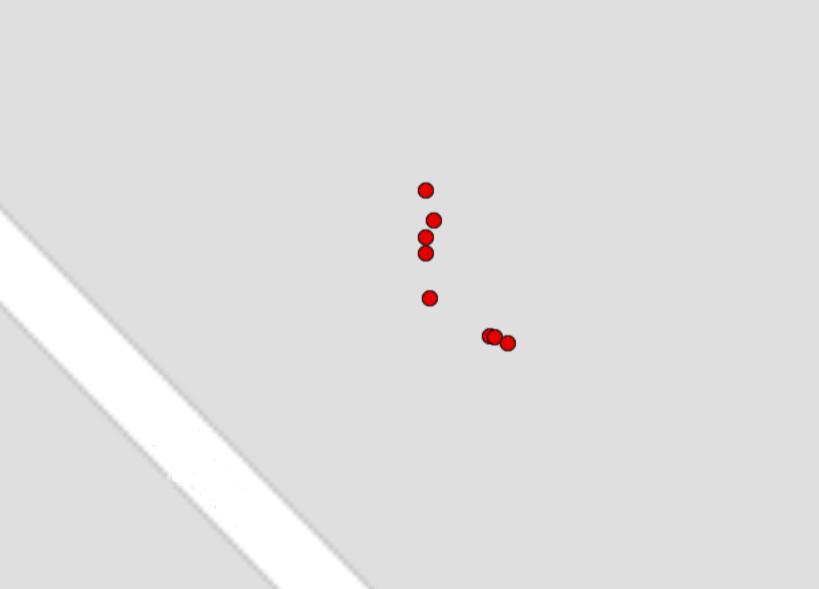
\includegraphics[width=3in]{img/mapka_punktygps.png}
\captionsetup{justification=centering}
\captionof{figure}{Wizualizacja współrzędnych nieporuszającego się odbiornika na mapie. [Opracowanie własne]}
\label{fig:mapka_punktygps}
}
\end{table}%

Zignorowanie powyższego zjawiska, mogłoby doprowadzić do bardzo niekorzystnej sytuacji. Gdyby osoba tworząca trasę zatrzymała się w trakcie treningu, na przykład w~celu odpoczynku lub zawiązania buta, zapisany przebieg treningu zawierałby skupisko fałszywych punktów. W celu wyeliminowania tego zagrożenia, podczas tworzenia trasy brane są pod uwagę tylko te punkty, które są oddalone od poprzedniego o więcej niż 15 metrów. Dzięki temu chwilowe zatrzymanie się podczas treningu, nie powoduje powstania przekłamań w~generowanej trasie.
\subsection{Zapobieganie oszustwom}\label{chap:zapobieganie-oszustwom}
Opieranie rywalizacji biegowej jednie na danych pobieranych z systemów nawigacji satelitarnej, sprawia że jej uczciwość może być zaburzona w stosunkowo łatwy sposób. Nic nie stoi na przeszkodzie, aby do pokonania trasy użyć chociażby roweru. Możliwe jest także manualne wprowadzanie danych lokalizacyjnych do urządzenia \cite{fakegps}, co pozwoli uzyskać dowolnie dobry wynik bez podejmowania jakiejkolwiek aktywności fizycznej. Zagrożenia tego można uniknąć na dwa sposoby:
\begin{itemize}
\item{\textbf{Porównywanie osiąganych przez użytkowników rezultatów z wynikami najlepszych na świecie biegaczy}} - Zapisanie w aplikacji zbioru światowych rekordów biegowych na konkretnych dystansach i porównywanie ich do wyników uzyskiwanych przez użytkowników jest pierwszym ze sposobów na zapobieganie oszustwom. Rezultaty znacząco lepsze od tych, które zostały osiągnięte na atestowanych zawodach z całą pewnością mogą zostać uznane jako osiągnięte nieuczciwie. Choć rozwiązanie to zapobiegnie zapisywaniu w rankingu czasów trasy, które są wręcz niemożliwe do osiągnięcia, nie sprawdzi się w przypadkach gdy sfałszowany wynik mieści się w granicach zdrowego rozsądku.
\item{\textbf{Skorzystanie z czujników dostępnych w urządzeniu}} - Akcelerometr oraz żyroskop są jednymi z wielu czujników umieszczanych w produkowanych obecnie telefonach komórkowych. Ich zadaniem jest mierzenie przyspieszenia liniowego oraz położenia kątowego \cite{czujniki}. Umożliwiają zatem pozyskanie informacji o ruchach jakim poddane jest urządzenie w trakcie trwania treningu. Opracowanie odpowiedniego algorytmu oraz skorzystanie z sieci neuronowych pozwoliłyby stwierdzić, czy dane pobrane z czujników w~czasie odbywania treningu, zgadzają się z tymi, które generowane są w czasie biegu i na tej podstawie dokonać akceptacji lub unieważnienia próby użytkownika. W~przeciwieństwie do poprzedniego podejścia, bieżące rozwiązanie okazałoby się skuteczne także w~przypadkach, w których dane lokalizacyjne zostały wprowadzone do urządzenia manualnie oraz gdy osiągnięty na trasie rezultat nie jest lepszy niż ogólnoświatowe rekordy. Rozwiązanie tego problemu obejmuje zagadnienia z dziedziny sztucznej inteligencji i wykracza poza zakres niniejszej pracy, dlatego też nie zostało zaimplementowane w tworzonej aplikacji.
\end{itemize}

\section{Istniejące rozwiązania w dziedzinie aplikacji treningowych}\label{chap:istniejace}
Na rynku aplikacji znajduje się wiele aplikacji, których przeznaczeniem jest wspieranie treningów biegowych. Pozwalają one użytkownikom na dogłębną analizę aktywności sportowych oraz śledzenie treningów zarówno swoich jak i udostępnianych przez innych biegaczy. Funkcjonalności te są bardzo powszechne. Nie udało się znaleźć aplikacji treningowej, która w pełni oferuje funkcjonalność zawartą w rozwiązaniu, które budowane jest w ramach niniejszej pracy, dlatego do niniejszego przeglądu wybrano trzy przykłady aplikacji, których zakres działania jest jak najbardziej do niej zbliżony, a jednocześnie cieszących się wysoką oceną oraz popularnością w sklepie z aplikacjami Google Play \cite{googleplay}. 
\subsection{Endomondo}
Jedną z najwcześniej wydanych (pierwsze wersja została udostępniona w listopadzie 2007 roku), a zarówno najbardziej popularnych na świecie aplikacji jest Endomondo \cite{endomondo}.  Pozwala na śledzenie aktywności w ponad 60 dyscyplinach sportowych, włączając w~to bieganie. W aplikacji rozwinięto aspekt społecznościowy - znajomi mają możliwość wzajemnego przeglądania historii swoich treningów. Ich statystyki mogą być także udostępniane na mediach społecznościowych. Ponadto istnieje możliwość tworzenia własnych tras, które inni biegacze mogą następnie przeglądać w formie listy i używać do własnych treningów. Niestety możliwe jest zobaczenie tylko całego zbioru tras, znajdujących się w pewnej nieznanej odległości od użytkownika. Stanowi to problem, ponieważ nie mogąc określić dokładnie obszaru wyszukiwania, biegacze nie są pewni, czy zobaczyli już wszystkie trasy, które mogłyby ich potencjalnie zainteresować czy może istnieje ich więcej, ale znajdują się poza nieznanym obszarem wyszukiwania. Producent nie udostępnił także możliwości filtrowania wyników wyszukiwania ze względu na długość trasy, twardość nawierzchni czy poziom terenu. Podczas tworzenia trasy zapisywana jest co prawda jej całkowita długość, jednak służy ona tylko poinformowaniu użytkownika, a nie wyszukiwaniu. Aplikacja nie pozwala także na jakiekolwiek porównywanie wyników, które biegacze osiągają na trasie.
\subsection{Strava}
Strava \cite{strava} jest aplikacją, która w momencie pisania niniejszej pracy wspiera treningi w~24 dyscyplinach sportowych. Oprócz podstawowej funkcjonalności aplikacji treningowych, oferuje także analizę treningów na podstawie rozmaitych statystyk i~wykresów. Aplikacja umożliwia także funkcję tworzenia i zapisywania tras. Oprócz samego jej przebiegu, zapisywana jest także jej długość oraz poziom terenu. Niestety, tak jak w przypadku aplikacji Endomondo, producent nie umożliwił filtrowania tras według żadnej z tych cech. Podczas przeglądania tras, ukazują się one na interaktywnej mapie, którą można przesuwać. Nie występuje tutaj zatem znany z Endomondo problem niemożności określenia obszaru, w którym wyszukiwane są trasy. Rozszerzenie obszaru poszukiwania ogranicza się do przesunięcia mapy na ekranie urządzenia. Zapisywanie czasów użytkowników którzy ukończyli trasę na serwerze, pozwala użytkownikom na wyświetlenie rankingu trasy i porównanie swojej dyspozycji do innych biegaczy. Funkcjonalność ta daje poczucie pewnego rodzaju rywalizacji, jednak sprawdzenie uzyskanego wyniku możliwe jest dopiero po ukończeniu treningu, użytkownik nie otrzymuje na ten temat informacji w czasie jego trwania.
\subsection{MapMyRun}
Przeznaczeniem aplikacji MapMyRun \cite{mapmyrun} jest przede wszystkim śledzenie aktywności związanych ze spacerowaniem i bieganiem. W tym przykładzie użytkownicy także mają możliwość przeglądania i analizowania swoich poprzednich treningów. Usprawnieniem jest fakt, iż trasy można filtrować na podstawie ich długości. Zabrakło niestety filtra poziomu terenu, mimo że informacja ta jest zapisywana podczas tworzenia trasy. Podczas wyszukiwania tras pojawia się problem znany z aplikacji Endomondo - prezentowane trasy należą do obszaru, którego granice oddalone są od użytkownika o~nieznaną odległość, przez co biegacze nie są pewni czy zostały im wyświetlone wszystkie godne uwagi trasy czy może część z nich znajduje się poza obszarem poszukiwań. Element rywalizacji jest zorganizowany podobnie jak w aplikacji Strava - wyniki osiągane przez użytkowników są zapisywane na serwerze, dzięki czemu mają oni możliwość sprawdzenia swojej dyspozycji po zakończonym treningu.
\chapter{Tworzenie i charakterystyka tras}\label{chap:charakterystyka-tras}
Tworzenie trasy polega na zapisaniu w systemie pozycji, ustalonych przy użyciu nawigacji satelitarnej, na których użytkownik znajdował się w trakcie treningu tak jak zostało to pokazane na rysunku przedstawiającym fragment utworzonej trasy \ref{image:mapka_fragment_trasy}, na którym linią ciągłą zaznaczono rzeczywistą trasę pokonaną przez biegacza, a kropkami reprezentację trasy zapisaną w systemie. Zapamiętywane są tylko te punkty, które znajdują się w odległości nie mniejszej niż 10 metrów od swojego poprzednika. Zaproponowana minimalna odległość pomiędzy punktami, pozwoli na osiągnięcie dostatecznie dokładnego przebiegu trasy, przy jednoczesnym zapobiegnięciu wystąpienia problemu, opisanego w rozdziale \ref{chap:wahania-pozycji}.

\begin{figure}[h]\label{fig:miary}
\begin{center}
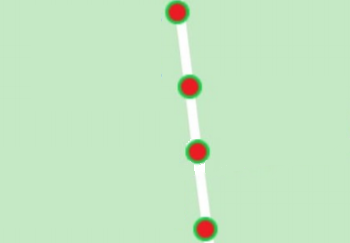
\includegraphics{img/mapka_fragment_trasy.png}
\caption{Fragment utworzonej trasy. [Opracowanie własne]}\label{image:mapka_fragment_trasy}
\end{center}
\end{figure}

Zawody biegowe w których biegacze biorą udział, różnią się trasami, na jakich są przeprowadzane. Ich dystans może wynosić od kilku do kilkudziesięciu kilometrów. Zawody odbywające się w mieście zwykle odbywają się na płaskiej nawierzchni asfaltowej, podczas gdy biegi organizowane w górach wymagają często od zawodników podbiegania pod jakiś szczyt górski lub zbiegania z niego. Nie inaczej jest z przygotowaniem do konkretnych zawodów. Chcąc jak najefektywniej przygotować się do startu, biegacz powinien trenować w warunkach zbliżonych do tych, które może spotkać na zawodach. Z tego względu aplikacja tworzona w ramach niniejszej pracy umożliwia użytkownikom wyszukiwanie tras treningowych, które spełnią ich preferencje. Niniejszy rozdział jest realizacją części pierwszego celu przedstawionego w rozdziale \ref{chap:cele-pracy}. Omówiono w nim cechy, które mogą zostać przypisane do trasy, sposób ich wyznaczenia na podstawie danych lokalizacyjnych oraz kryteria wyszukiwania używane podczas przeglądania tras. 
\section{Możliwe cechy trasy}\label{chap:opis-cech}
Do każdej trasy mogą zostać przypisane 3 cechy.
\begin{itemize}
\item{\textbf{Dystans}} - określa jak długa jest trasa. Wartość wyrażona jest w kilometrach.
\item{\textbf{Poziom terenu}} - Reprezentuje zmianę wysokości nad poziomem morza pomiędzy początkiem a końcem trasy. Wartości które może przyjąć ta cecha to:
\begin{itemize}
\item{Wyrównany} - gdy wysokość nad poziomem morze nie zmienia się lub zmienia się nieznacznie,
\item{Rosnący} - gdy wysokość nad poziomem morza wzrasta,
\item{Malejący} - gdy wysokość nad poziomem morza maleje.
\end{itemize}
\item{\textbf{Twardość nawierzchni}} - Wyraża jaka część całej trasy przebiega przez nawierzchnię utwardzoną (na przykład asfalt lub kostka brukowa) w stosunku do nawierzchni nieutwardzonej (na przykład piasek lub trawa). Wartość wyrażona jest w procentach. Przykładowo wartość 60\% dla trasy o dystansie 10 kilometrów oznacza, że 6 kilometrów prowadzi przez nawierzchnię utwardzoną, a 4 kilometry przez nieutwardzoną.
\end{itemize}
\section{Przypisanie cech do trasy}
Długość trasy przypisywana jest bezpośrednio po ukończeniu treningu. Jej wyznaczenie polega na zsumowaniu odległości pomiędzy wszystkimi następującymi po sobie punktami przy użyciu wzorów \ref{eq:haversine1},  \ref{eq:haversine2} i \ref{eq:haversine3}.

Określenie poziomu terenu odbywa się poprzez obliczenie różnicy wysokości nad poziomem morza pomiędzy punktem rozpoczynającym oraz kończącym trasę i przypisanie odpowiednio poziomu:
\begin{itemize}
\item{\textbf{wyrównanego}} - gdy różnica nie przekracza 10\%,
\item{\textbf{rosnącego}} - gdy wysokość punktu końcowego jest większa od wysokości punktu początkowego o więcej niż 10\%,
\item{\textbf{malejącego}} - gdy wysokość punktu początkowego jest większa od wysokości punktu końcowego o więcej niż 10\%.
\end {itemize}
Należy mieć na uwadze, że w przypadku wystąpienia problemu opisanego w rozdziale \ref{chap:problem-poziom-terenu}, cecha ta będzie musiała zostać ustalona przez użytkownika.

W celu umożliwienia automatycznego przypisania rodzaju nawierzchni, posłużono się serwisem OpenStreetMap \cite{osm}. Narzędzie to pozwala scharakteryzować podłoże ustalonego przez klienta obszaru. Musi on być zdefiniowany w formie prostokąta, a odbywa się to poprzez dostarczenie serwisowi współrzędnych geograficznych jego lewej dolnej oraz prawej górnej krawędzi. Zdefiniowane przykładowego obszaru zostało pokazane na rysunku \ref{image:mapka_obszar}. Kropkami oznaczono podane współrzędne geograficzne, natomiast linia ciągła definiuje obszar, który zostanie poddany analizie. W odpowiedzi klient otrzymuje charakterystykę wszystkich dróg, które znalazły się w zdefiniowanym obszarze \cite{osm-docs-wiki}. Rodzaj nawierzchni nie jest zwracany w formie „utwardzona” bądź „nieutwardzona”, lecz w formie sprecyzowanej, na przykład „asfalt” lub „trawa”, dlatego pierwszym krokiem którego trzeba się podjąć po otrzymaniu odpowiedzi, jest przyporządkowanie etykiety  „utwardzona” bądź „nieutwardzona” dla każdego z otrzymanych obiektów. Przyporządkowanie wszystkich możliwych do otrzymania rodzajów nawierzchni zostało pokazane w tabeli \ref{table:rodzaje-nawierzchni} \cite{osm-surface}.

\begin{figure}[h]\label{fig:miary}
\begin{center}
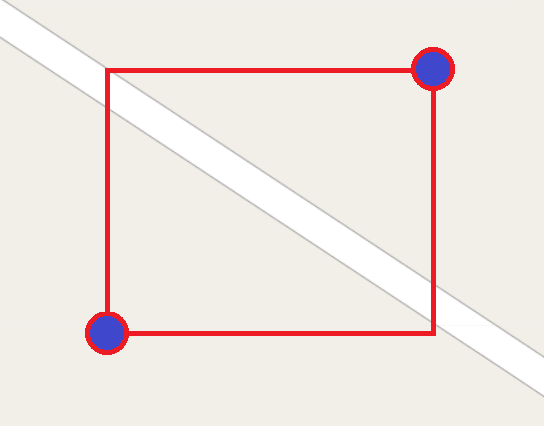
\includegraphics[width=2in]{img/mapka_obszar.png}
\caption{Obszar poddany analizie [Opracowanie własne]}\label{image:mapka_obszar}
\end{center}
\end{figure}

\begin{table}[thb]
\caption{Przyporządkowanie konkretnego rodzaju nawierzchni do jej reprezentacji w tworzonym systemie \cite{osm-surface}}.\label{table:rodzaje-nawierzchni}
\centering\renewcommand\cellalign{lc}
\setcellgapes{3pt}\makegapedcells
\begin{tabular}{|c|c|} \hline
\textbf{Nawierzchnia utwardzona} & \textbf{Nawierzchnia nieutwardzona} \\ \hline
\makecell{paved, asphalt, concrete,\\concrete:lanes, concrete:plates,\\paving\textunderscore stones, sett,\\unhewn\textunderscore cobblestone,\\cobblestone, metal, wood,\\metal\textunderscore grid } & \makecell{ unpaved, compacted, fine\textunderscore gravel,\\gravel, pebblestone, dirt,\\earth, grass, grass\textunderscore paver,\\ground, mud, sand, woodchips,\\snow, ice, salt, clay, tartan,\\artifical\textunderscore turf, decoturf, carpet} \\ \hline
\end{tabular}
\end{table}

Tworzone przez użytkowników trasy zapisywane są w formie punktów, dlatego przed skorzystaniem z serwisu OpenStreetMap, należy zdefiniować wspomniany prostokątny obszar poszukiwań. Korzystając ze wzoru \cite{eq:haversine_generowanie_punktu} wyznaczane są więc 2 nowe punkty: oddalony o 10 metrów i 225 stopni względem północy oraz oddalony o 10 metrów i 45 stopni względem północy. Po ustaleniu rodzaju nawierzchni dla każdego z punktów trasy, możliwe jest wyliczenie wartości procentowej, a tym samym określenie cechy według wzoru:
\begin{equation}\label{eq:haversine1}
{Twardość\hspace{0.15cm} nawierzchni} = \frac{u}{u + n} \cdot 100,
\end{equation}
gdzie \(u\) oznacza liczbę obiektów z etykietą  „utwardzona”, \(n\) liczbę obiektów z etykietą  „nieutwardzona”.
Z uwagi na czytelność wynik zaokrąglany jest do liczby całkowitej.
Należy mieć na uwadze, że OpenStreetMap jest projektem tworzonym przez społeczność i dla pewnych dróg rodzaj nawierzchni mógł być przypisany błędnie bądź nie przypisany wcale. Wartość określonej cechy powinna być zatem traktowana w formie propozycji, którą użytkownik tworzący trasę może poprawić wedle własnego uznania.

\section{Kryteria wyszukiwania tras}
Kryteria wyszukiwania są ściśle powiązane z cechami opisanymi w rozdziale \ref{chap:opis-cech}. Dokonano jedynie kilku usprawnień mających na celu wygodę użytkownika.
\begin{itemize}
\item{Kryterium \textbf{długości trasy} przyjmuje wartości „od” oraz „do”. Oznacza to, że lista wynikowa zawiera trasy nie krótsze niż pierwsza z nich, a jednocześnie nie dłuższe niż druga z nich. Największa wartość, którą można określić wynosi 20 kilometrów.  Po jej przekroczeniu, przy wyszukiwaniu pod uwagę brane są trasy o nieograniczonej maksymalnej długości,}
\item{Przy filtrowaniu ze względu na \textbf{poziom terenu} oprócz konkretnych wartości cechy możliwe jest także wybranie opcji „każdy”. Oznacza to, że trasy nie będą filtrowane według tej cechy.}
\item{\textbf{Twardość nawierzchni} podobnie jak w przypadku długości trasy określana jest jako zakres  „od, do”. Wartość maksymalna wynosi 100\%.}
\end{itemize}
Oprócz tego użytkownik musi określić maksymalny promień wyszukiwania względem jego obecnej lokalizacji. Dzięki temu jest on świadomy, że zostały mu pokazane wszystkie trasy z interesującego go obszaru. Nie bez znaczenia jest także fakt, że zapobiegnie to pobieraniu z bazy danych wszystkich istniejących tras, co miałoby znaczący wpływ na wykorzystanie łącza oraz wydajność zarówno aplikacji serwerowej jak i aplikacji mobilnej.
\chapter{Symulacja rywalizacji na podstawie zgromadzonych danych}\label{chap:symulacja-rywalizacji}
Funkcja wirtualnej rywalizacji daje użytkownikom uczucie uczestniczenia w~prawdziwych zawodach. Współzawodnictwo z innymi biegaczami może sprawić, że trening będzie nie tylko efektywniejszy, ale także przyjemniejszy. Jest też rozwiązaniem dla osób, które chcą sprawdzić swoją dyspozycję bez ponoszenia kosztów podróży oraz wpisowego na prawdziwe zawody. Ponadto ze względu, że w wirtualnym wyścigu „bierze udział” także najlepszy poprzedni czas użytkownika na danej trasie, ma on możliwość zweryfikowania, czy jego forma staje się lepsza. Niniejszy rozdział jest kontynuacją realizacji pierwszego celu przedstawionego w~rozdziale \ref{chap:cele-pracy}. Omówiono rozwiązanie problemu wirtualnej rywalizacji oraz opisano w jaki sposób użytkownik informowany jest o zachodzących w trakcie wyścigu zdarzeniach.
\section{Sposób przeprowadzenia procesu wirtualnej rywalizacji}\label{chapter:sposob-rywalizacji}
W momencie gdy użytkownik wybierze jedną z udostępnionych przez społeczność tras i~rozpocznie trening, punkty których przeznaczeniem było do tej pory jedynie reprezentowanie przebiegu trasy, przyjmują rolę punktów kontrolnych. Zadaniem biegacza chcącego wziąć udział w wirtualnej rywalizacji, jest przebiegnięcie obok wszystkich punktów w kolejności, w~której zostały one stworzone. Przebieg takiego treningu musi więc pokrywać się z przebiegiem treningu użytkownika, który stworzył trasę. Aby następny w kolejności punkt kontrolny został oznaczony jako „osiągnięty”, odległość pomiędzy aktualną pozycją użytkownika, a pozycją punktu kontrolnego obliczona za pomocą wzorów \ref{eq:haversine11},  \ref{eq:haversine2} i \ref{eq:haversine3} musi być nie większa niż 10 metrów.

Za każdym razem gdy punkt kontrolny zostaje „osiągnięty”, zapisywany jest aktualny czas użytkownika. Zapisywanie osiągniętego czasu ma miejsce również podczas tworzenia trasy w~momencie zapisywania pozycji punktów. Oznacza to, że osoba tworząca trasę jako pierwsza dodawana jest do jej rankingu.

Posiadając dane o czasach użytkowników na każdym z punktów kontrolnych trasy, możliwe jest przeprowadzenie procesu wirtualnej rywalizacji. Wraz z rozpoczęciem treningu użytkownik „osiąga” pierwszy punkt kontrolny (będący jednocześnie pierwszym punktem zapisanej trasy). W tym momencie zostaje on dodany na koniec rankingu. Sytuacja ta została przedstawiona w tabeli \ref{table:rywalizacja1} oraz na rysunku \ref{fig:rywalizacja1}. Trójkątny kształt oznacza pozycję użytkownika, natomiast kropki reprezentują punkty kontrolne. Za~każdym razem gdy biegacz „osiąga” następny w~kolejności punkt kontrolny, ranking aktualizowany jest tak, aby wskazywać aktualnie przez niego zajmowaną pozycję. Oznacza to, że miejsce w rankingu może (choć nie musi) zmieniać się za każdym razem, gdy osiągnięty jest punkt kontrolny. Sytuacja zmiany pozycji została przedstawiona w~tabeli \ref{table:rywalizacja2} oraz na rysunku \ref{fig:rywalizacja2}.  Ostatni punkt kontrolny jest jednocześnie końcowym punktem trasy, a więc osiągnięcie go doprowadza do wyznaczenia końcowego rankingu trasy.

\begin{table}[h!]
\parbox{\dimexpr\linewidth-6cm\relax}{\centering%
\captionsetup{justification=centering}
\captionof{table}{Ranking na początku rywalizacji biegowej.}\label{table:rywalizacja1}
\begin{tabular}{|c|c|}
\hline
%\textbf{L.p.} & \textbf{Szerokość \newline geograficzna} & \textbf{Długość geograficzna} \\
 \begin{tabular}[c]{@{}c@{}}Zajmowana\\pozycja\end{tabular} & \begin{tabular}[c]{@{}c@{}}Użytkownik\end{tabular} \\
\hline
1 & Użytkownik A\\\hline
2 & Użytkownik B\\\hline
3 & Użytkownik C\\\hline
\rowcolor{GREEN}
4 & Bieżący użytkownik\\\hline
\end{tabular}
\label{tab:xt}}
\parbox{6cm}{%
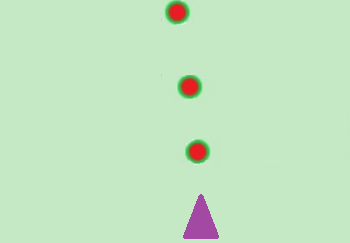
\includegraphics[width=2in]{img/rywalizacja1.png}
\captionsetup{justification=centering}
\captionof{figure}{Początek rywalizacji biegowej [Opracowanie własne]}
\label{fig:rywalizacja1}
}
\end{table}%

\begin{table}[h!]
\parbox{\dimexpr\linewidth-6cm\relax}{\centering%
\captionsetup{justification=centering}
\captionof{table}{Ranking po „osiągnięciu” kolejnego punktu kontrolnego.}\label{table:rywalizacja2}
\begin{tabular}{|c|c|}
\hline
%\textbf{L.p.} & \textbf{Szerokość \newline geograficzna} & \textbf{Długość geograficzna} \\
 \begin{tabular}[c]{@{}c@{}}Zajmowana\\pozycja\end{tabular} & \begin{tabular}[c]{@{}c@{}}Użytkownik\end{tabular} \\
\hline
1 & Użytkownik B\\\hline
2 & Użytkownik A\\\hline
\rowcolor{GREEN}
3 & Bieżący użytkownik\\\hline
4 & Użytkownik C\\\hline
\end{tabular}
\label{tab:xt}}
\parbox{5cm}{%
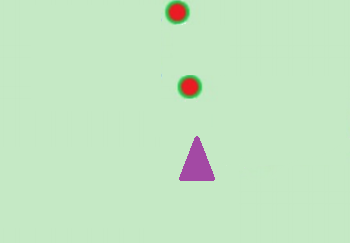
\includegraphics[width=2in]{img/rywalizacja2.png}
\captionsetup{justification=centering}
\captionof{figure}{Rywalizacja biegowa po osiągnięciu kolejnego punktu [Opracowanie własne]}
\label{fig:rywalizacja2}
}
\end{table}%

Tak jak zostało wspomniane we wstępie do niniejszego rozdziału, użytkownik ma możliwość rywalizacji „ze samym sobą”, a więc oprócz próby obecnej w rankingu może znajdować się także próba biegacza dodana w czasie treningu odbytego wcześniej. Takie zjawisko może mieć jednak miejsce tylko w czasie trwania treningu. Oznacza to, że po jego zakończenia musi zajść jeden z następujących scenariuszy:
\begin {itemize}
\item{użytkownik nie odbył wcześniej treningu w ramach trasy - bieżąca próba jest zapisywana w~systemie},
\item{użytkownik odbył wcześniej trening w ramach trasy, a jego końcowy rezultat był lepszy niż w próbie bieżącej - bieżąca próba zostaje odrzucona},
\item{użytkownik odbił wcześniej trening w ramach trasy, a jego końcowy rezultat był gorszy niż w próbie bieżącej - bieżąca próba zastępuje w systemie próbę poprzednią}.
\end{itemize}
\section{Informowanie użytkownika o rezultatach}\label{chap:zasada-tts}
Podstawowym sposobem informowania biegacza jest wyświetlanie stanu treningu na ekranie urządzenia. Użytkownik ma do dyspozycji interaktywną mapę na której pokazana jest jego aktualna pozycja oraz wszystkie punkty kontrolne. Za każdym razem gdy następny w~kolejności punkt kontrolny zostanie osiągnięty, zostaje on usunięty z mapy, aby użytkownik był świadom, że może udać się w kierunku kolejnego. Ponadto na ekranie wyświetlony jest ranking bieżącej rywalizacji biegowej. Przedstawia on czasy na ostatnio osiągniętym punkcie kontrolnym oraz nazwy użytkownika wszystkich biegaczy, których próba zapisana jest w~systemie. Miejsca w rankingu aktualizowane są za każdym razem gdy biegacz, który odbywa trening, osiągnie następny punkt kontrolny.

Biegacze często korzystają w czasie treningu z zestawu słuchawkowego. Wobec tego w~celu zwiększenia immersji płynącej z wirtualnej rywalizacji, użytkownik informowany jest o~rezultatach poprzez odtworzenie głosowych komunikatów. Za każdym razem gdy użytkownik osiągnie punkt kontrolny odtwarzana jest informacja:
\begin{itemize}
\item{\textbf{o aktualnie zajmowanej pozycji}, gdy pozycja zajmowana na właśnie osiągniętym punkcie kontrolnym jest taka sama jak na poprzednim punkcie kontrolnym},
\item{\textbf{o liczbie zdobytych pozycji}, gdy pozycja zajmowana na właśnie osiągniętym punkcie kontrolnym jest lepsza niż na poprzednim punkcie kontrolnym},
\item{\textbf{o liczbie utraconych pozycji}, gdy pozycja zajmowana na właśnie osiągniętym punkcie kontrolnym jest słabsza niż na poprzednim punkcie kontrolnym}.
\end{itemize}
\chapter{Zastosowane technologie}\label{chap:zastosowane-technologie}
W niniejszym rozdziale opisane zostały technologie użyte podczas tworzenia zarówno aplikacji mobilnej jak i aplikacji webowej.
\section{Oprogramowanie}
\textbf{Visual Studio Community 2019}\cite{visual-studio} - Zintegrowane środowisko programistyczne wydane przez firmę Microsoft \cite{microsoft}. Choć pozwala na pracę z wieloma językami programowania, jego przeznaczeniem jest głównie tworzenie oprogramowania w języku C\# \cite{csharp}. Visual Studio pozwala także na generowanie kodu, wykonywanie operacji bezpośrednio na serwerze bazodanowym, pracę z systemami kontroli wersji oraz korzystanie z wielu udogodnień wspomagających pracę programisty. Istnieje także możliwość dodatkowego rozszerzenia funkcjonalności środowiska programistycznego za pomocą oddzielnych rozszerzeń. Dzięki wsparciu dla wielu technologii, możliwe jest tworzenie oprogramowania o rozmaitym przeznaczeniu, zaczynając od programów przeznaczonych na komputery i urządzenia mobilne, przez aplikacje webowe, aż po gry wideo i rozwiązania wykorzystujące nauczanie maszynowe.

Tworzony w Visual Studio program podzielony jest na \textbf{projekty} (ang. \textit{projects}). Każdy projekt reprezentuje niezależny, oddzielnie kompilowany kod źródłowy. Zbiór projektów, które ze sobą współpracują są zwykle grupowane w jedno \textbf{rozwiązanie} (ang. \textit{solution}). Pozwala ono programistom w łatwy sposób dodawać lub usuwać projekty a także zarządzać procesem ich kompilacji.

\section{Aplikacja mobilna}
Do stworzenia części mobilnej budowanego systemu wybrano technologię \textbf{Xamarin} \cite{xamarin_docs}, wydaną przez firmę Microsoft. Wykorzystuje ona kod pisany w języku C\# do implementacji logiki aplikacji oraz kod XML \ref{xml} do tworzenia interfejsów użytkownika. Zdecydowano się na ten wybór przede wszystkim z powodu możliwości budowy aplikacji wieloplatformowych, jakie udostępnia ta technologia. Jest to szczególnie ważne, ponieważ pomimo że w obecnej fazie aplikacja jest przeznaczona tylko na urządzenia mobilne z systemem operacyjnym Android \cite{android}, zakłada się, że w przyszłości może ona wspierać także system operacyjny iOS \ref{ios} oraz inteligentne zegarki.

Istnieją dwa podejścia budowania aplikacji wieloplatformowych w Xamarin:
\begin {itemize}
\item{Xamarin Forms} - Pozwala współdzielić kod źródłowy odpowiadający zarówno za logikę aplikacji jak i interfejs użytkownika. Podczas tworzenia interfejsu możliwe jest używanie tylko pewnego zbioru kontrolek, które korzystają z natywnych funkcjonalności wspólnych dla wszystkich obsługiwanych w Xamarin systemów operacyjnych \cite{xamarin-forms}. 
\item{Xamarin Native} - Pozwala współdzielić kod źródłowy odpowiadający za logikę. interfejs użytkownika tworzony jest dla każdego systemu operacyjnego oddzielnie. Dzięki temu w aplikacji mogą być wykorzystywane wszystkie funkcje udostępniane przez system operacyjny \cite{xamarin-native}.
\end{itemize}
W celu uniknięcia problemów z obsługą nawigacji satelitarnej, wyświetlaniem rankingu oraz punktów kontrolnych na mapie w tworzonym rozwiązaniu użyto podejścia Native, a więc kontrolki używane w widokach aplikacji, są kontrolkami należącymi bezpośrednio do systemu Android.

\section{Aplikacja webowa}
Do stworzenia części serwerowej budowanego systemu wybrano język C\# oraz szkielet aplikacyjny (ang. \textit{framework}) \textbf{ASP.NET Core} służący do budowy aplikacji internetu rzeczy, aplikacji internetowych, programów działających w chmurze obliczeniowej czy (co istotne w tym przypadku) części serwerowych aplikacji mobilnych. ASP.NET Core został wydany w 2016 roku jako nowa i udoskonalona odsłona szkieletu aplikacyjnego ASP.NET. Nowa wersja zapewnia wieloplatformowość (aplikacje mogą być tworzone i uruchamiane w systemach Windows, Linux i macOS). Ważną cechą tej technologii jest nastawienie na wydajność - w przeciwieństwie do swojego poprzednika ASP.NET Core nie jest oparty na jednej bibliotece, ale na zestawie pakietów zawierających różnorodne funkcjonalności. Dzięki temu do aplikacji dodane są tylko te zależności, które rzeczywiście są używane, a w efekcie jest ona bardziej wydajna \cite{ksiazka-asp-core}.

Komunikacja pomiędzy aplikacją serwerową a bazą danych odbywa się poprzez bibliotekę \textbf{Entity Framework}, która jest platformą mapowania obiektowo-relacyjnego. Pozwala ona zastąpić konieczność pisania kodu SQL (\textit{Structured Query Language}) \cite{sql} wykonywaniem operacji bazodanowych poprzez modyfikowanie stanu obiektów w programie.

\section{System zarządzania bazą danych}
Jako oprogramowanie odpowiedzialne za zapisywanie, odczytywanie oraz zarządzanie danymi wybrano \textbf{SQL Server}. Jest to system zarządzania relacyjną bazą danych wydany przez firmę Microsoft. SQL Server jest jednym z najczęściej stosowanych rozwiązań w tej dziedzinie. Swoją pozycję zawdzięcza sobie wysoką wydajnością, ścisłą integracją z pozostałymi produktami Microsoft (na przykład chmurą Azure), łatwością w instalacji i eksploatacji (istnieją dedykowane narzędzia, które znacznie upraszczają zarządzania bazami danych)  \cite{ksiazka-sql}.

\section{Obsługa map}
W systemie posłużono się dwoma różnymi rozwiązaniami oferującymi obsługę i dostęp do mapy świata.
\subsection{Wyświetlanie mapy w aplikacji mobilnej}
Mapa wyświetlana jest na ekranie urządzenia mobilnego dzięki wykorzystaniu biblioteki serwisu \textbf{Google Maps} \cite{google-maps}. Charakteryzuje się ona wysokim poziomem interaktywności. Użytkownik ma możliwość przesuwania, oddalania, przybliżania mapy oraz śledzenia własnej pozycji. Programista ma także możliwość wyświetlania na mapie rozmaitych grafik takich jak: ikony, linie, figury geometryczne, markery i personalizowania jej według własnych potrzeb.

W chwili pisania niniejszej pracy dostęp do wymienionych funkcjonalności jest całkowicie darmowy. Dodatkowej opłaty wymagają funkcje związane z wskazywaniem drogi do konkretnego punktu oraz pokazywaniem szczegółowych informacji o konkretnych lokalizacjach \cite{google-maps-pricing}.
\subsection{Automatyczne ustalanie twardości nawierzchni}
\textbf{OpenStreetMap} \cite{osm} jest projektem mającym na celu stworzenie darmowej mapy całego globu. Mapa jest tworzona przez społeczność. Oznacza to, że każdy ma możliwość modyfikowania jej i wprowadzania poprawek. Dane mogą być aktualizowane na podstawie odczytów z systemów nawigacji satelitarnej, innych map lub na podstawie własnych doświadczeń. Istotną cechą mapy jest jej szczegółowość. W jej tworzeniu bierze udział wiele osób i to od nich samych zależy jakie informacje zostaną umieszczone na mapie. W efekcie oprócz dróg i budynków można na niej znaleźć nawet takie obiekty jak skrzynki pocztowe, żywopłoty czy bocianie gniazda. \cite{osm-gather-data}. 

OpenStreetMap udostępnia także programistom możliwość pozyskania danych poprzez kierowanie do serwisu zapytań HTTP. Funkcjonalność ta została użyta w aplikacji dostarczanej w ramach niniejszej pracy do określania twardości terenu na tworzonej trasie. Aspekt ten opisano w rozdziale \ref{chap:przypisanie-cech}. Oprócz charakterystyki rodzaju terenu w odpowiedziach otrzymywanych z serwisu można znaleźć także wszystkie inne informacje, które użytkownicy uwzględnili tworząc konkretny fragment mapy. Przyjmuje się, że bezpieczna ilość zapytań, którą można kierować do serwisu bez jego obciążenia wynosi 10000 \cite{osm-docs-wiki}.
\chapter{Dokumentaja techniczna}\label{chap:dokumentacja-techniczna}
Niniejszy rozdział stanowi objaśnienie, w jaki sposób system został stworzony. Zawiera opis wymagań oraz szczegóły implementacyjne dotyczące budowy poszczególnych warstw przy wykorzystaniu technologii opisanych w rozdziale \ref{chap:zastosowane-technologie}.
\section{Projekt systemu}
\subsection{Opis założeń}
moja-aplikacja składa się z aplikacji przeznaczonej na urządzenia z systemem Android \cite{android} oraz wspierającej ją aplikacji webowej. Komunikacja pomiędzy nimi odbywa się poprzez protokół HTTP (\textit{Hypertext Transfer Protocol}), a sam interfejs aplikacji serwerowej został wykonany w stylu \textbf{REST} (\textit{Representational state transfer}). Oznacza to między innymi, że konkretny zasób na serwerze jest identyfikowany na podstawie przypisanego mu URI (\textit{Uniform Resource Identifier}), a użytkownik odpytujący serwer jest identyfikowany na podstawie parametru zawartego w nagłówkach żądania. Wymiana danych pomiędzy obiema aplikacjami odbywa się przy pomocy formatu JSON (\textit{JavaScript Object Notation}). \cite{ksiazka-asp-core}

\subsubsection{Aplikacja mobilna powinna:}
\begin{itemize}
\item{Wspierać wieloplatformość} - zastosowana architektura powinna oddzielać logikę biznesową aplikacji od interfejsu graficznego. W efekcie dzięki zastosowaniu technologii Xamarin, przeniesienie aplikacji na inny mobilny system operacyjny powinno ograniczać się do zbudowania jedynie widoku przeznaczonego pod ten system.
\item{Pozwalać użytkownikom tworzyć trasy, a także umożliwiać manualne lub automatyczne określenie ich cech.}
\item{Pozwalać przeglądać trasy na podstawie zdefiniowanych przez użytkownika kryteriów wyszukiwania.}
\item{Pozwalać na przeprowadzenie treningu na wybranej trasie wraz z elementem wirtualnej rywalizacji.}
\item{Informować użytkownika o rezultatach zarówno poprzez informacje wyświetlane na ekranie jak i odtwarzane głosowo.}
\item{Reagować na błędy - na przykład nieudane połączenie z aplikacją serwerową.}
\end{itemize}

\subsubsection{Aplikacja serwerowa powinna:}
\begin{itemize}
\item{Pozwolić wyszukiwać trasy na podstawie otrzymanych kryteriów}
\item{Zapisywać trasy stworzone przez użytkowników}
\item{Zapisywać próby użytkowników na trasach}
\end{itemize}

\subsection{Podział projektu}
Dzięki skorzystaniu z technologii umożliwiającej tworzenie aplikacji mobilnych, aplikacji serwerowych oraz zintegrowanego środowiska programistycznego pochodzącego od jednego producenta, możliwe było tworzenie obu aplikacji w ramach pojedynczego rozwiązania (ang. \textit{solution}). Pozwoliło to na pisanie kodu źródłowego, kompilowanie oraz uruchamianie w trybie debugowania obu aplikacji w jednym momencie. Nie było więc potrzeby korzystania z dwóch różnych środowisk programistycznych jednocześnie, co okazało się bardzo znaczącym udogodnieniem w kontekście wydajnościowym.

Stworzona solucja zawiera następujące projekty:
\begin{itemize}
\item{Api} - zawiera część serwerową systemu.
\item{Core} - zawiera logikę biznesową oraz model danych części aplikacji mobilnej systemu.
\item{MobileAndroid} - zawiera kod interfejs użytkownika aplikacji przeznaczonej na system operacyjny Android.
\end{itemize}
Rozdzielenie logiki biznesowej oraz modelu danych od widoku aplikacji mobilnej sprawia, że dodanie wsparcia dla dodatkowych mobilnych systemów operacyjnych ogranicza się do stworzenia w solucji nowego projektu zawierającego jedynie interfejs użytkownika oraz wykorzystanie projektu Core do jego obsługi.

\subsection{Przygotowanie aplikacji do działania}
\subsubsection{Aplikacja serwerowa}
Przed zbudowaniem aplikacji serwerowej należy ustawić w pliku konfiguracyjnym projektu (\textit{appsettings.json}) parametry połączenia (ang \textit{connection string}) bazy danych. Przykład konfiguracji przedstawiono na listingu \ref{listing:appsettings}.

\begin{lstlisting}[caption={Plik konfiguracyjny aplikacji serwerowej},label=listing:appsettings]
{
  "ConnectionStrings": {
    "Default": "data source=.SQLEXPRESS; initial catalog=
    BscThesisDb; integrated security=SSPI"
  }
}
\end{lstlisting}

Następnie należy wykonać polecenie \textit{dotnet build}. Spowoduje ono pobranie potrzebnych zależności oraz zbudowanie projektu. Ostatnim krokiem jest wywołanie polecenia \textit{dotnet ef database update} w celu stworzenia bazy danych i potrzebnych tabel.

\subsubsection{Aplikacja mobilna}
Przed zbudowaniem aplikacji mobilnej należy ustawić wartość zmiennej \textit{ApiBaseAddress} w klasie \textit{WebRepositoryBase} znajdującej się w projekcie \textit{Core} w przestrzeni nazw \textit{Repositories.Web}. Przechowuje ona adres pod jakim znajduje się uruchomiona instancja części serwerowej systemu. Pod zdefiniowany adres będą więc kierowane wszystkie zapytania HTTP wychodzące z aplikacji mobilnej. Przykładowo zdefiniowany adres przedstawiono na listingu \ref{listing:webrepobase}.

\begin{lstlisting}[caption={Klasa zawierająca adres aplikacji serwerowej},label=listing:webrepobase]
public abstract class WebRepositoryBase
{
	private const string ApiBaseAddress = 
		"http://192.168.1.16:5000/";
	protected readonly HttpClient Client;

	protected WebRepositoryBase()
	{
		Client = new HttpClient { BaseAddress =
			new Uri(ApiBaseAddress) };
	}
}
\end{lstlisting}

Po wykonaniu tej czynności należy pobrać zależności i zbudować aplikację za pomocą polecenia \textit{dotnet build}.


\section{Warstwa modelu danych}
Informacje o trasach i wynikach przesyłane są z aplikacji mobilnej do serwerowej, a więc klasy reprezentujące model danych w obu projektach pokrywają się w znacznej części.
\subsection{Aplikacja mobilna}\label{chap:model-mobilna}
Zaprojektowany model danych zgodnie z założeniami pozwala na wyznaczenie oraz przechowywanie cech charakteryzujących trasę. Jego reprezentacja w formie diagramu klas została przedstawiona na rysunku \ref{image:xamarin_model}. Pierwszoplanową rolę w modelu danych odgrywa klasa \textit{Route}, będąca główną reprezentacją trasy. Sama w sobie nie przechowuje ona żadnych danych z wyjątkiem identyfikatora trasy w systemie, jednak zawiera odwołania do pozostałych klas:
\begin{itemize}
\item{\textit{Point}} - Przechowuje informacje o pojedynczym punkcie z którego składa się trasa. Warto zauważyć, że typ danych właściwości (ang. {property}) pozwala na przypisanie wartości \textit{null}. Spowodowane jest to faktem, iż istnieje prawdopodobieństwo posiadania informacji o szerokości i długości geograficznej nie znając jednocześnie wysokości nad poziomem morza. Zjawisko to zostało opisane w rozdziale \ref{chap:problem-poziom-terenu}. Do każdego punktu przypisany jest także jego numer oznaczający kolejność w której występuje na trasie.
\item{\textit{RouteProperties}} - Przechowuje nazwę oraz cechy trasy, a więc dystans, poziom twardości nawierzchni oraz poziom nachylenia terenu będący typem wyliczeniowym.
\item{\textit{RankingRecord}} - Przechowuje informacje o próbach użytkowników na trasie. Czasy osiągane na poszczególnych punktach kontrolnych zapisane są we właściwości \textit{CheckpointTimes} będącej kolekcją. Jej \textit{i-ty} element przechowuje liczbę sekund, która upłynęła od rozpoczęcia treningu w momencie „osiągnięcia” \textit{i-tego} punktu kontrolnego. Oprócz tego w klasie znajdują się właściwości identyfikujące trasę oraz użytkownika oraz pozwalające stwierdzić czy konkretna próba na trasie należy do aktualnie zalogowanego użytkownika (\textit{IsMine}) oraz czy oznacza aktualnie trwającą próbę (\textit{IsCurrentTry}).
\end{itemize}
\begin{figure}[h]\label{fig:xamarin_model}
\begin{center}
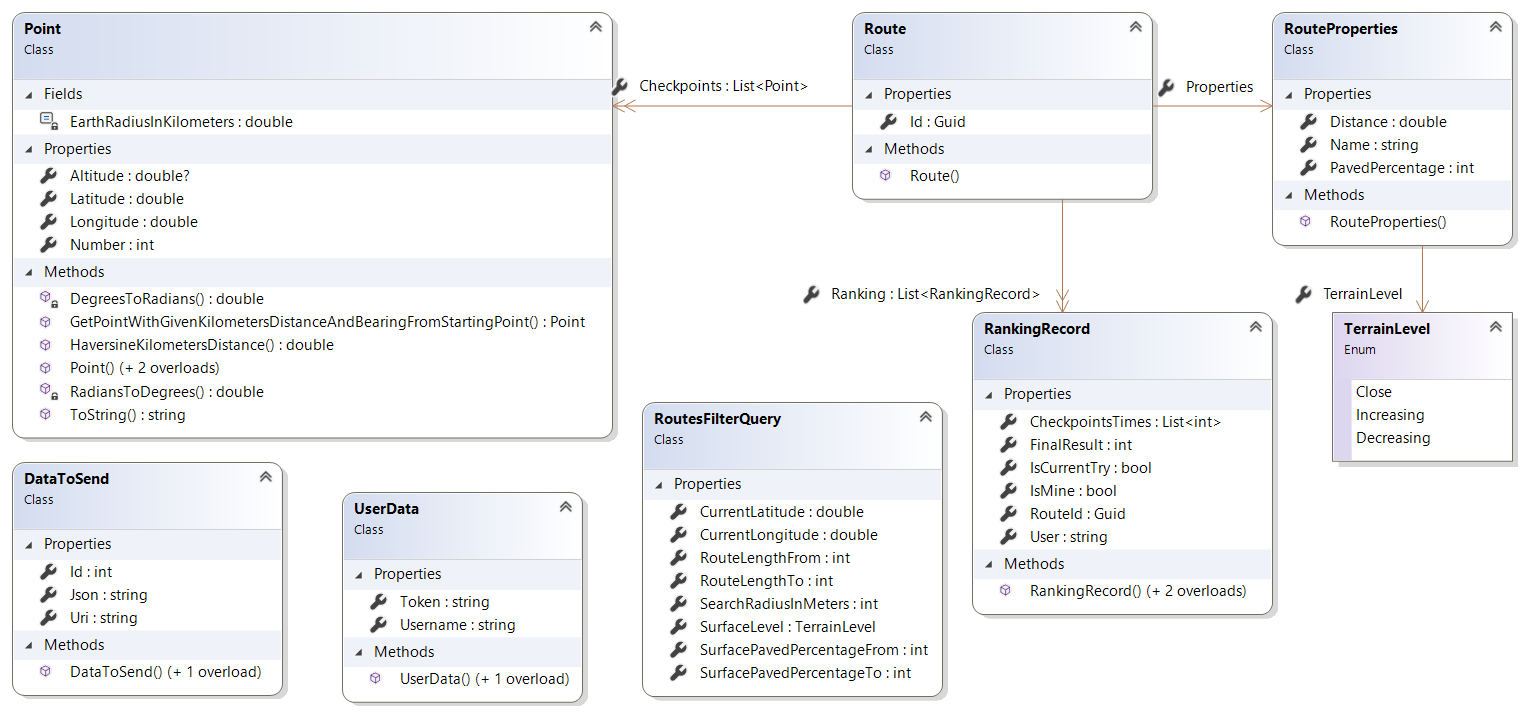
\includegraphics[width=\textwidth]{img/xamarin_model.png}
\caption{Diagram klas modelu danych aplikacji mobilnej [Opracowanie własne]}\label{image:xamarin_model}
\end{center}
\end{figure}
Ponad to model danych zawiera dwie dodatkowe klasy:
\begin{itemize}
\item{\textit{DataToSend}} - przechowuje dane w formacie JSON oraz adres URL. Pozwala podjąć ponowną, odłożoną w czasie próbę wysłania danych na serwer w przypadku gdy proces ten nie zakończy się sukcesem przy pierwszym podejściu.
\item{\textit{UserData}} - przechowuje dane o aktualnie zalogowanym użytkowniku: login użytkownika oraz token używany podczas komunikacji z serwerem.
\end{itemize}
\subsection{Aplikacja serwerowa}
Z racji podobieństwa do modelu danych zawartego w aplikacji mobilnej, który opisany został w rozdziale \ref{chap:model-mobilna}, w rozdziale niniejszym zostaną przybliżone jedynie nie omówione wcześniej aspekty. 

\begin{figure}[h]\label{fig:api_model}
\begin{center}
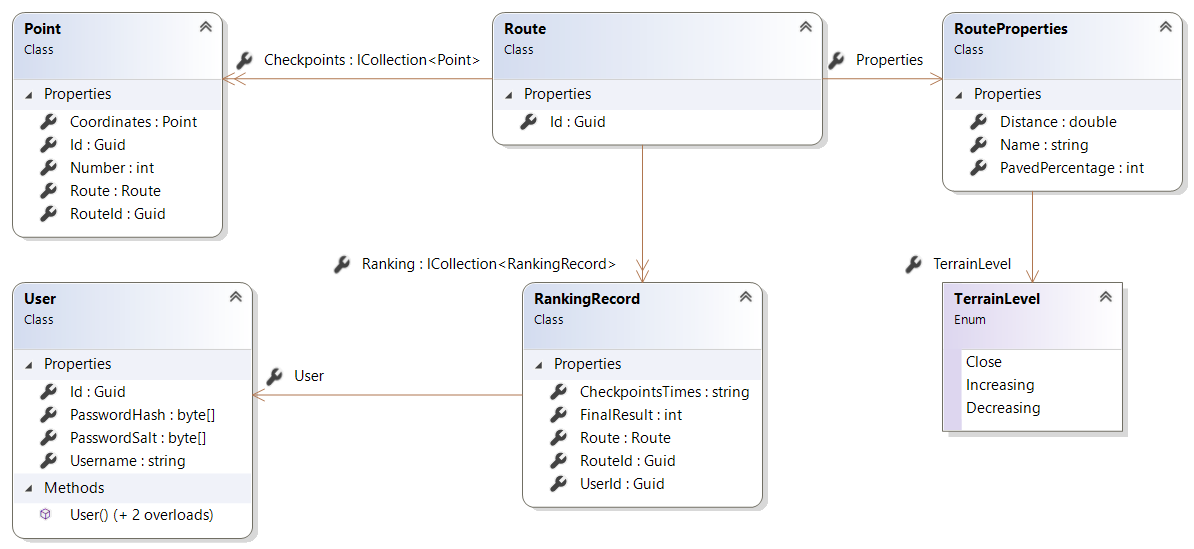
\includegraphics[width=\textwidth]{img/api_model.png}
\caption{Diagram klas modelu danych aplikacji serwerowej [Opracowanie własne]}\label{image:api_model}
\end{center}
\end{figure}

Jak widać na diagramie \ref{image:api_model} w modelu aplikacji serwerowej istnieje klasa \textit{User}. Reprezentuje ona konto użytkownika w systemie. Powiązanie tej klasy z klasą reprezentującą próbę na trasie, pozwala określić do którego z użytkowników należy konkretny wynik.

Współrzędne punktów trasy zapisywane przy użyciu typu danych \textit{Point}. Należy zaznaczyć, że nie jest to typ stworzony w ramach modelu danych, lecz należącą do przestrzeni nazw \textit{NetTopologySuite.Geometries}, występującą w środowisku .NET reprezentacją typu \textit{geography} istniejącego w systemie zarządzania bazą danych SQL Server. \textit{Geography} pozwala na przechowywanie współrzędnych geograficznych punktu (wraz z wysokością nad poziomem morza) w jednej kolumnie tabeli bazodanowej. \cite{geography-type}

\begin{figure}[h]
\begin{center}
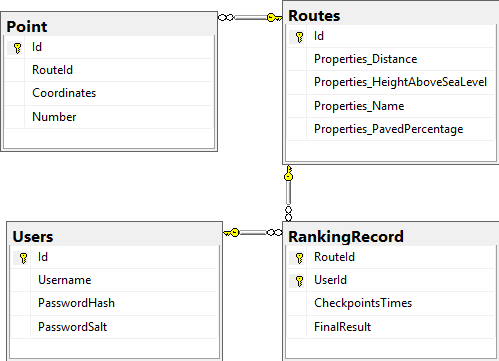
\includegraphics{img/er-diagram.png}
\caption{Diagram encji bazy danych [Opracowanie własne]}\label{image:db-structure}
\end{center}
\end{figure}

Zastosowanie mapowania obiektowo-relacyjnego pozwoliło na odwzorowanie modelu danych w formie bazy danych. Jej struktura została przedstawiona na rysunku \ref{image:db-structure}. Przed utworzeniem odpowiednich tabel konieczne było zdefiniowanie relacji pomiędzy polami tabel. Odpowiednią konfigurację umieszczono w klasie \textit{Context} znajdującej się w przestrzeni nazw \textit {Api.Entities} i przedstawiono na listingu \ref{listing:context}.

\begin{lstlisting}[caption={Konfiguracja mapowania relacyjno-obiektowego},label=listing:context]
protected override void OnModelCreating(
ModelBuilder modelBuilder)
{
    modelBuilder.Entity<Route>().HasMany(r => r.Checkpoints)
    	.WithOne(cp => cp.Route)
    	.HasForeignKey(cp => cp.RouteId);
    modelBuilder.Entity<Route>().OwnsOne(r => r.Properties);
    modelBuilder.Entity<Route>().HasMany(r => r.Ranking)
    	.WithOne(rr => rr.Route)
        .HasForeignKey(rr => rr.RouteId);

    modelBuilder.Entity<RankingRecord>().HasOne(rr => rr.User);
    modelBuilder.Entity<RankingRecord>()
    	.HasKey(rr => new { rr.RouteId, rr.UserId });

    base.OnModelCreating(modelBuilder);
}
\end{lstlisting}
Konfiguracja pozwoliła na utworzenie następujących relacji:
\begin{itemize}
\item{jeden do wielu pomiędzy tabelami reprezentującymi klasy \textit{Route}} oraz \textit{Point}
\item{jeden do wielu pomiędzy tabelami reprezentującymi klasy \textit{Route}} oraz \textit{RankingRecord}
\item{jeden do jednego pomiędzy tabelami reprezentującymi klasy \textit{RankingRecord} oraz \textit{User}}
\end{itemize}
Dzięki instrukcji z linii numer 7 dane z klas \textit{Route} oraz \textit{RouteProperties} zostały umieszczone w jednej tabeli. Pozwoliło to na uniknięcie łączenia tabel podczas pobierania danych. Typy wyliczeniowe nie wymagają osobnej tabeli i są przechowywane w postaci liczb, dlatego nie było potrzeby tworzenia dodatkowej struktury dla cechy \textit{poziom terenu}.

Warto zauważyć, że czasy osiągane na punktach kontrolnych są przechowywane jako łańcuch znaków (\textit{string}). Pozwoliło to uniknąć tworzenia dodatkowej tabeli i relacji jeden do wielu z tabelą reprezentującą klasę \textit{RankingRecord}. Mapowanie pomiędzy kolekcją a łańcuchem znaków odbywa się w klasie \textit{AutomapperConfig} znajdującej się w przestrzeni nazw \textit{Api.Mappers} i zostało przedstawione na listingu \ref{listing:collection-string-mapping}.
\begin{lstlisting}[caption={Mapowanie pomiedzy kolekcją a łańcuchem znaków},label=collection-string-mapping]
public static IMapper Initialize()
    => new MapperConfiguration(cfg =>
        {
         cfg.CreateMap<RankingRecord, RankingRecordDto>()
             .ForMember(dest => dest.CheckpointsTimes, opt =>
                    opt.MapFrom(src => src.CheckpointsTimes
                    .Split(" ", StringSplitOptions.None).Select(int.Parse)))
         cfg.CreateMap<RankingRecordDto, RankingRecord>()
             .ForMember(dest => dest.CheckpointsTimes,
                 opt => opt.MapFrom(src => 
                 string.Join(" ", src.CheckpointsTimes)))
        })
        .CreateMapper();
\end{lstlisting}

\section{Warstwa logiki biznesowej}
\subsection{Wyszukiwanie tras}
Wyszukiwanie tras odbywa się poprzez wysłanie zapytania z aplikacji mobilnej do aplikacji serwerowej. Ustalone przez użytkownika kryteria wyszukiwania są następnie przekazywane do bazy danych. Dzięki temu proces odfiltrowania tras ma miejsce tak wcześnie jak to możliwe i do aplikacji serwerowej, a następnie mobilnej trafiają tylko te trasy, które rzeczywiście spełniają ustalone kryteria. Diagram sekwencji tego procesu został pokazany na rysunku \ref{image:sekwencja_wyszukiwanie}. Kryteria wybrane przez użytkownika zapisane są w instancji klasy \textit{RoutesFilterQuery}, która pozwala zachować wszystkie informacje opisane w rozdziale \ref{chap:kryteria}. Obiekt ten jest przekazywany do części serwerowej systemu w celu dokonania odpowiedniej filtracji tras.

W momencie gdy zostanie wywołana metoda \textit{GetRoutesAsync} klasy \textit{RoutesRepository}, przekazany obiekt jest wykorzystany do określenia warunków, które muszą spełniać pobierane trasy. Działanie to zostało pokazane na listingu \ref{listing:filtracja_tras}. Warto podkreślić, że dzięki zastosowaniu typu \textit{geography} w tabeli bazy danych, możliwe jest policzenie odległości pomiędzy pozycją użytkownika a początkiem trasy bezpośrednio na poziomie bazy danych \cite{geography-type, geography-type2}. Warunek ten określa linia numer 8 listingu. Na podstawie określonych warunków generowane jest następnie zapytanie SQL wykonywane bezpośrednio na poziomie bazy danych.
\begin{lstlisting}[caption={Określenie warunków dla pobieranych tras},label=listing:filtracja_tras]
var routes = _context.Routes
	 .Where(r => r.Properties.PavedPercentage 
         >= query.SurfacePavedPercentageFrom
	&& r.Properties.PavedPercentage <= query.SurfacePavedPercentageTo)
        .Where(r => r.Properties.Distance >= query.RouteLengthFrom
        && r.Properties.Distance <= query.RouteLengthTo)
        .Where(r => r.Checkpoints.First(cp => cp.Number == 0)
        .Coordinates.IsWithinDistance(currentLocation,
        query.SearchRadiusInMeters));

if (query.SurfaceLevel > 0)
	routes = routes.Where(r => r.Properties.TerrainLevel 
	== (TerrainLevel)query.SurfaceLevel);
\end{lstlisting}
\begin{figure}[h]\label{fig:api_model}
\begin{center}
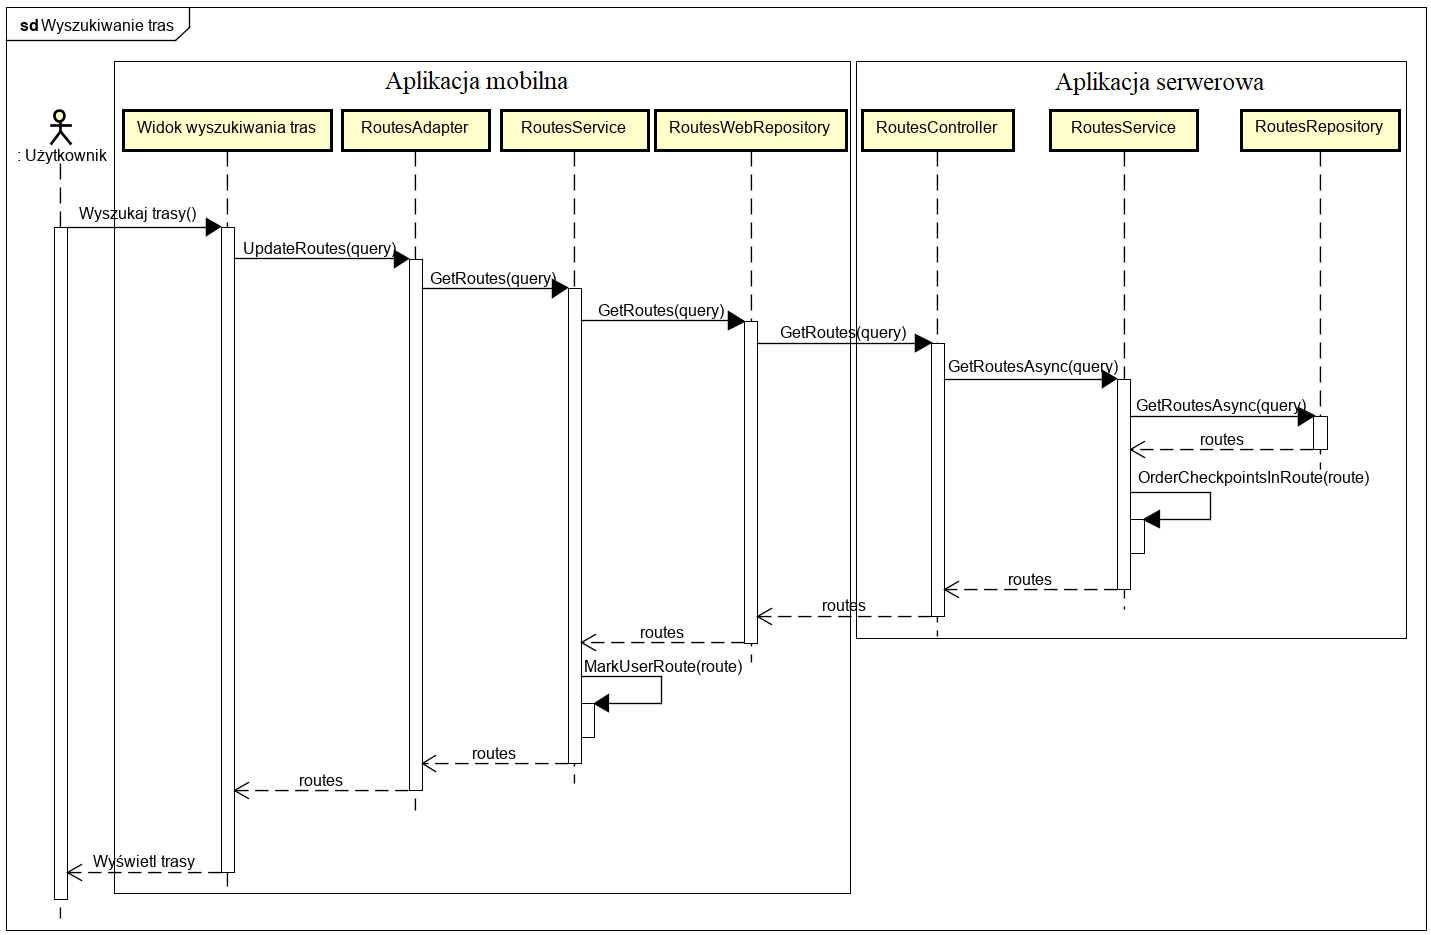
\includegraphics[width=\textwidth]{img/diagram_sekwencji_wyszukiwanie.png}
\caption{Diagram sekwencji procesu wyszukiwania tras [Opracowanie własne]}\label{image:sekwencja_wyszukiwanie}
\end{center}
\end{figure}
Po pobraniu danych z bazy danych, w klasie \textit{RoutesService} z przestrzeni nazw \textit{Api.Services} aplikacji serwerowej punkty kontrolne każdej trasy są sortowane według własciwości \textit{Number}, tak aby ich kolejność w kolekcji odpowiadała kolejności, którą powinny zajmować na trasie. Oprócz tego pozycje rankingowe są sortowane według właściwości \textit{FinalResult}, dzięki czemu w momencie przejścia do szczegółów trasy, użytkownik widzi jej końcowy ranking. Po przesłaniu danych o trasach z aplikacji serwerowej do aplikacji mobilnej, w klasie \textit{RoutesService} znajdującej się przestrzeni nazw \textit{Core.Services}, odbywa się aktualizacja właściwości \textit{IsMine}. Proces ten został pokazany na listingu \ref{listing:ismine}. Dzięki temu w interfejsie użytkownika możliwe jest wyróżnienie wyniku, który należy do biegacza.
\begin{lstlisting}[caption={Aktualizacja właściwości IsMine klasy Route},label=listing:ismine]
private void MarkUserRoute(Route route)
{
	var mineRankingRecord = route.Ranking
	.FirstOrDefault(r => r.User == _userData.Username);
	if (mineRankingRecord != null)
		mineRankingRecord.IsMine = true;
}
\end{lstlisting}

\subsection{Odbywanie treningu}\label{chap:trening}
Implementacje treningu, który tworzy nową trasę jak i trening przeprowadzany w ramach istniejącej trasy, który zawiera w sobie dodatkowo element wirtualnej rywalizacji zawierają wspólną logikę, dlatego tak jak widać na rysunku \ref{image:trening-diagram}, skorzystano z mechanizmu dziedziczenia. Należy zwrócić uwagę, że klasy te zawierają kilka pól typu \textit{Action}. Dzięki nim możliwe jest aktualizowanie interfejsu użytkownika z poziomu metody klasy należącej do logiki biznesowej. W przypadku stworzenia aplikacji mobilnej przeznaczonej na inny system operacyjny, wystarczy przekazać odpowiednie implementacje metod odpowiedzialnych za aktualizację interfejsu użytkownika, a zostaną one wywołane. 

Metody \textit{Start} oraz \textit{Stop} służą do odpowiednio do rozpoczęcia i zakończenia treningu. Zawierają one logikę odpowiedzialną za dodanie obecnej próby użytkownika do rankingu oraz uruchomienie i zatrzymanie stopera. Dzięki stoperowi za każdym razem gdy upłynie jedna sekunda, aktualizowany jest interfejs użytkownika oraz wywoływana jest metoda \textit{ProcessUserLocation}, której implementacja zależna jest od typu treningu.
\begin{figure}[h]\label{fig:asdl}
\begin{center}
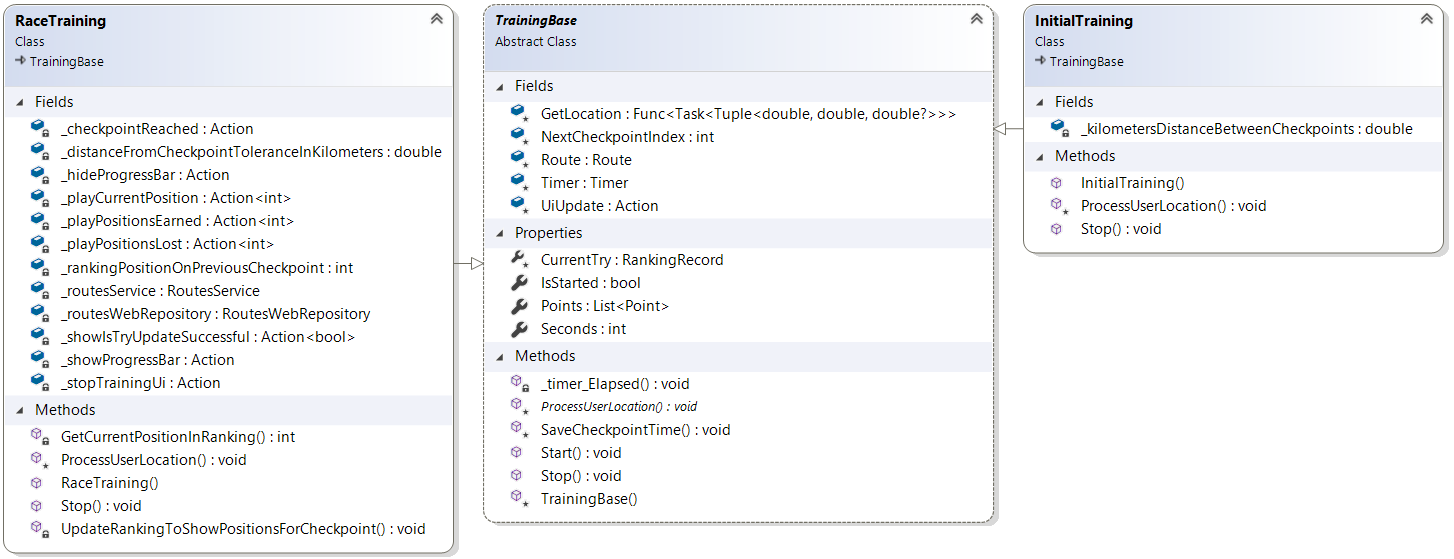
\includegraphics[width=\textwidth]{img/trening-diagram.png}
\caption{Diagram klas odpowiadających za przeprowadzanie treningów [Opracowanie własne]}\label{image:trening-diagram}
\end{center}
\end{figure}
\subsubsection{Trening tworzący trasę}
Za logikę obsługującą trening na nowej trasie odpowiada klasa \textit{InitialTraining}. Za każdym razem gdy wywołana zostanie metoda \textit{ProcessUserLocation}, podejmowana jest próba dodania do tworzonej trasy nowego punktu kontrolnego na podstawie obecnej pozycji biegacza. Aby punkt mógł zostać dodany, użytkownik musi znajdować się w pozycji nie mniejszej niż 10 metrów od ostatnio utworzonego punktu kontrolnego. Prawdziwość tego warunku jest sprawdzana w linii numer 6, 7 i 8 na listingu \ref{listing:add-point-initial}. Działanie ma to na celu uniknięcie problemu opisanego w rozdziale \ref{chap:wahania-pozycji}, którego wystąpienie spowodowałoby utworzenie skupiska punktów kontrolnych oddalonych od siebie o kilka metrów. Wyznaczenie odległości pomiędzy aktualną pozycją użytkownika, a ostatnio utworzonym punktem kontrolnym obliczana jest za pomocą formuły Haversine przytoczonej w rozdziale \ref{chap:haversine}. Jej implementacja została pokazana na listingu \ref{listing:haversine}. Współrzędne odczytywane są w stopniach, dlatego przed obliczeniem odległości, konieczne było wyznaczenie ich wartości w radianach.
\begin{lstlisting}[caption={Wyznaczenie odległości pomiędzy dwoma punktami},label=listing:haversine]
public static double HaversineKilometersDistance(Point point1,
	Point point2)
{
  var latitudeDelta = DegreesToRadians(point1.Latitude - point2.Latitude);
  var longitudeDelta = DegreesToRadians(
  	point1.Longitude - point2.Longitude);

  var firstPointLatitudeCos = Math.Cos(DegreesToRadians(point1.Latitude));
  var secondPointLatitudeCos = Math.Cos(
  	DegreesToRadians(point2.Latitude));

  var a = Math.Pow(Math.Sin(latitudeDelta / 2), 2)
  	+ firstPointLatitudeCos *
	secondPointLatitudeCos * Math.Pow(Math.Sin(longitudeDelta / 2), 2);
  var c = 2 * Math.Atan2(Math.Sqrt(a), Math.Sqrt(1 - a));
  var d = EarthRadiusInKilometers * c;

  return d;
}
\end{lstlisting}

\begin{lstlisting}[caption={Tworzenie punktów kontrolnych},label=listing:add-point-initial]
protected override async void ProcessUserLocation()
{
    var location = await GetLocation();
    var currentPosition = new Point(
    	location.Item1, location.Item2,location.Item3,NextCheckpointIndex);
    var distanceFromLastPoint = Route.Checkpoints.Any()
        ? Point.HaversineKilometersDistance(Route.Checkpoints.Last(),
        currentPosition)
        : _kilometersDistanceBetweenCheckpoints;
    if (distanceFromLastPoint >= _kilometersDistanceBetweenCheckpoints)
    {
        NextCheckpointIndex++;
        Route.Checkpoints.Add(currentPosition);
        SaveCheckpointTime();
    }
}
\end{lstlisting}
Wraz z utworzeniem punktu kontrolnego, zapisywany jest także czas, który upłynął od rozpoczęcia treningu. Oznacza to, że biegacz tworzący trasę, zostaje jednocześnie pierwszym użytkownikiem dodanym do rankingu.

W momencie gdy użytkownik postanawia zakończyć trening, wywołana zostaje metoda \textit{Stop}. Oprócz bazowej implementacji tej metody, zostaje także wykonany kod odpowiedzialny za utworzenie ostatniego punktu kontrolnego. Jest on tworzony niezależnie od odległości do przedostatniego punktu kontrolnego, a jego pozycja odpowiada pozycji użytkownika z momentu zakończenia treningu.

\subsubsection{Trening na zapisanej trasie oraz wirtualna rywalizacja}
Proces wirtualnej rywalizacji odbywa się wraz z rozpoczęciem treningu na stworzonej wcześniej trasie. Za obsługę obu tych elementów odpowiada klasa \textit{RaceTraining}. Metoda \textit{ProcessUserLocation} służy do zapisywania czasów, które biegacz osiągnął na każdym z punktów kontrolnych. Jej kod źródłowy został przedstawiony na listingu \ref{listing:add-point-race}.
\begin{lstlisting}[caption={Proces wirtualnej rywalizacji},label=listing:add-point-race]
protected override async void ProcessUserLocation()
{
  var location = await GetLocation();
  var currentLocation = (new Point(location.Item1,
    location.Item2, Seconds));
  var distance = Point.HaversineKilometersDistance(currentLocation,
    Route.Checkpoints[NextCheckpointIndex]);

  if (distance < _distanceFromCheckpointToleranceInKilometers)
  {
      NextCheckpointIndex++;

      SaveCheckpointTime();
      if (NextCheckpointIndex == Route.Checkpoints.Count)
      {
        Stop();
        _routesService.ProcessCurrentTry(Route, CurrentTry);

        _stopTrainingUi.Invoke();

        _showProgressBar.Invoke();
        var isSuccessful = await _routesWebRepository
		.CreateRankingRecordAsync(CurrentTry, Route.Id);
        _hideProgressBar.Invoke();
        _showIsTryUpdateSuccessful.Invoke(isSuccessful);
      }
      else
      {
        UpdateRankingToShowPositionsForCheckpoint(NextCheckpointIndex - 1);

        var currentPosition = GetCurrentPositionInRanking();
        if (currentPosition == 
          rankingPositionOnPreviousCheckpoint
            || _rankingPositionOnPreviousCheckpoint == 0)
        {
            _playCurrentPosition.Invoke(currentPosition);
        }
        else
        {
            if (currentPosition < _rankingPositionOnPreviousCheckpoint)
                _playPositionsEarned(
                _rankingPositionOnPreviousCheckpoint
                  - currentPosition);
            else
                _playPositionsLost(currentPosition
                  - _rankingPositionOnPreviousCheckpoint);
         }

        _rankingPositionOnPreviousCheckpoint = currentPosition;

        _checkpointReached.Invoke();
      }
  }
}
\end{lstlisting}
Biegacz musi znajdować się w odległości nie większej niż 10 metrów od następnego w kolejności punktu kontrolnego. Gdy ten warunek zostanie spełniony, bieżący czas od rozpoczęcia treningu zostaje zapisany. Odległość pomiędzy użytkownikiem a punktem kontrolnym wyznaczana jest za pomocą formuły haversine, której implementacja znajduje się na listingu \ref{listing:haversine}. Za każdym razem gdy punkt kontrolny zostanie osiągnięty, aktualizowany jest ranking. Odbywa się to poprzez posortowanie kolekcji \textit{Ranking} znajdującej się w instancji klasy \textit{Route} względem wartości, która reprezentuje czas osiągnięty przez wszystkich użytkowników na punkcie kontrolnym. Oprócz faktu, że pozycje w rankingu wyświetlonym na ekranie urządzenia zmieniają się wraz z trwaniem biegu, odtwarzane są komunikaty głosowe. Logika odpowiadająca za ten proces znajduje się w liniach 32-47 listingu \ref{listing:add-point-race} i jest implementacją warunków opisanych w rozdziale \ref{chap:zasada-tts}.

W momencie gdy zostaną osiągnięte wszystkie punkty kontrolne, trening jest automatycznie zakańczany, a próba użytkownika jest poddawana przetworzeniu. Scenariusz ten realizują linie 15-26 listingu \ref{listing:add-point-race}. Proces przetworzenia próby jest implementacją warunków opisanych w rozdziale \ref{chapter:sposob-rywalizacji} i został przedstawiony na listingu \ref{listing:przetworzenie-proby}.
\begin{lstlisting}[caption={Przetworzenie próby użytkownika},label=listing:przetworzenie-proby]
public void ProcessCurrentTry(Route route, RankingRecord currentTry)
{
    var lastTry = route.Ranking.SingleOrDefault(rr => rr.IsMine);
    if (lastTry == null) 
        return;
    if (currentTry.FinalResult < lastTry.FinalResult)
    {
        currentTry.IsMine = true;
        currentTry.IsCurrentTry = false;
        currentTry.User = lastTry.User;

        route.Ranking.Remove(lastTry);
    }
    else
        route.Ranking.Remove(currentTry);
}
\end{lstlisting}
Logika ta jest wykonywana na urządzeniu mobilnym, dzięki czemu użytkownik ma możliwość sprawdzenia końcowego rankingu wirtualnej rywalizacji. Warto zaznaczyć, że próba jest także wysyłana do aplikacji serwerowej, gdzie przetwarzana jest w ten sam sposób. Ma to miejsce nawet w przypadku, gdy końcowa lokata użytkownika w rankingu na urządzeniu mobilnym nie zmieniła się. Jest to spowodowane brakiem gwarancji, że ranking zapisany w bazie danych, jest nadal w tym samym stanie, co w momencie pobrania go na urządzenie mobilne przed rozpoczęciem treningu.

\subsection{Automatyczne przypisywanie cech do trasy}
Logikę odpowiedzialną za automatyczne przypisywanie cech umieszczono w klasie \textit{RoutesService}, która znajduje się w przestrzeni nazw \textit{Core.Services}. Została zaimplementowana zgodnie z opisem zawartym w rozdziale \ref{chap:przypisanie-cech}.
\subsubsection{Długość trasy}
Wyznaczenie długości polega na zsumowaniu odległości pomiędzy wszystkimi punktami trasy przy pomocy formuły haversine, której implementację pokazano na listingu \ref{listing:haversine}.
\begin{lstlisting}[caption={Wyznaczenie długości trasy},label=listing:dlugosc-trasy]
public void CalculateRouteDistance(Route route)
{
    var totalDistance = 0d;
    for (int i = 0; i < route.Checkpoints.Count - 1; i++)
    {
        totalDistance += Point.HaversineKilometersDistance(
        	route.Checkpoints[i], route.Checkpoints[i + 1]);
    }
    route.Properties.Distance = Math.Round(totalDistance, 2);
}
\end{lstlisting}
\subsubsection{Poziom terenu}
Wyznaczenie poziomu terenu zostało pokazane na listingu \ref{listing:poziom-terenu}. Wartość zmiennej \textit{terrainLevelDifferenceThresholdInPercentage} wyraża maksymalną procentową różnicę pomiędzy wysokością początkową a końcową dla której poziom terenu będzie uznany jako wyrównany. W tym przypadku wynosi ona 10\%.

Ponadto poziom terenu zostanie wyznaczony jako „wyrównany”, gdy nie udało się wyznaczyć wysokości któregokolwiek z punktów.
\begin{lstlisting}[caption={Wyznaczenie poziomu terenu},label=listing:poziom-terenu]
private void ResolveTerrainLevel(Route route)
{
    const int terrainLevelDifferenceThresholdInPercentage = 10;
    const double terrainLevelDifferenceThreshold =
    	1.0 * terrainLevelDifferenceThresholdInPercentage / 100 + 1;
    var startAltitude = route.Checkpoints.First().Altitude;
    var finishAltitude = route.Checkpoints.Last().Altitude;

    route.Properties.TerrainLevel = TerrainLevel.Close;
    if (startAltitude != null && finishAltitude != null)
    {
        if (startAltitude 
        	> finishAltitude * terrainLevelDifferenceThreshold)
        {
            route.Properties.TerrainLevel = TerrainLevel.Decreasing;
        }
        else if (finishAltitude 
        	> startAltitude * terrainLevelDifferenceThreshold)
        {
            route.Properties.TerrainLevel = TerrainLevel.Increasing;
        }
    }
}
\end{lstlisting}
\subsubsection{Twardość nawierzchni}
Za wyznaczenie tej cechy odpowiada klasa \textit{OsmService}. Główna metoda odpowiedzialna za to działanie została przedstawiona na listingu \ref{listing:twardosc-nawierzchni}. Metoda wywoływana w linii numer 3 listingu zajmuje się zbudowaniem odpowiedniego zapytania zgodnie z zasadami opisanymi w \cite{overpass-wiki}, wysłaniem go do serwisu OpenStreetMap \cite{osm} oraz zwróceniem otrzymanej odpowiedzi. W efekcie do zmiennej \textit{tags} zostają przypisane rodzaje nawierzchni dla każdego punktu trasy, natomiast zmienne \textit{PavedSurfaces} oraz \textit{UnpavedSurfaces} zawierają wszystkie możliwe utwardzone oraz nieutwardzone rodzaje nawierzchni zgodnie z tabelą \ref{table:rodzaje-nawierzchni} z rozdziału \ref{chapter:wyznaczenie-twardosc}. Na tej podstawie w liniach 4-7 wyznaczana jest procentowa twardość nawierzchni utworzonej trasy. 
W przypadku gdy nie uda się ustalić twardość nawierzchni (na przykład gdy z zewnętrznego serwisu nie uda się otrzymać żadnych informacji) twardość trasy zostaje ustalona jako wartość zmiennej \textit{DefaultSurfacePavement} wynosząca 50\%.
\begin{lstlisting}[caption={Wyznaczenie poziomu terenu},label=listing:twardosc-nawierzchni]
public async Task<int> ResolveRouteSurfaceTypeAsync(Route route)
{
  var tags = (await GetSurfaceTypesAsync(route.Checkpoints)).ToList();
  int pavedCount = tags.Count(t => PavedSurfaces.Contains(t));
  int unpavedCount = tags.Count(t => UnpavedSurfaces.Contains(t));

  var pavedPercent = 1.0 * pavedCount / (pavedCount + unpavedCount) * 100;
  if (double.IsNaN(pavedPercent))
      return DefaultSurfacePavement;

  return (int)Math.Round(pavedPercent);
}
\end{lstlisting}

\subsection{Brak połączenia z serwerem po zakończonym treningu}
Może zdarzyć się, że nie uda się zapisać treningu użytkownika, ponieważ urządzenie nie miało dostępu do internetu lub nastąpiła awaria serwera. W takim wypadku użytkownik utraciłby swoją próbę. Aby tego uniknąć, w momencie gdy nie uda się nawiązać połączenia z serwerem, dane o treningu w formacie JSON oraz adres pod który miały być wysłane zapisywane są w lokalnej bazie danych urządzenia. Następnie możliwe jest podjęcie ponownej próby wysłania zaległych danych. Proces ten został przedstawiony na listingu \ref{listing:overdue-data}. Metoda \textit{ProcessOverdueData} wywoływana jest przy każdym uruchomieniu aplikacji. Z lokalnej bazy danych pobierane są wszystkie zaległe treningi, a następnie po raz kolejny wysłane do części serwerowej aplikacji w metodzie wywoływanej w linii numer 6 listingu. W przypadku powodzenia tej operacji trening jest usuwany z lokalnej bazy danych.
\begin{lstlisting}[caption={Wyznaczenie poziomu terenu},label=listing:overdue-data]
public async Task ProcessOverdueData()
{
    var dataToSend = _userLocalRepository.GetDataToSend();
    foreach (var data in dataToSend)
    {
        var result = await _routesWebRepository
        	.SendJsonData(data.Json, data.Uri);

        if (result)
            _userLocalRepository.DeleteDataToSend(data.Id);
    }
}
\end{lstlisting}

\section{Warstwa interfejsu użytkownika}
Za warstwę interfejsu użytkownika odpowiada aplikacja przeznaczona dla systemu operacyjnego Android \cite{Android}. Aby możliwe było korzystanie z aplikacji, użytkownik musi udzielić jej pozwolenia na wykorzystanie nawigacji satelitarnej. 
\subsection{Wyszukiwanie tras}
Widok wyszukiwania tras składa się z części odpowiedzialnej za umożliwienie użytkownikowi wybranie omówionych w rozdziale \ref{chap:kryteria} kryteriów wyszukiwania oraz części która wyświetla znalezione trasy w formie listy.

Ustalone kryteria wyszukiwania przypisywane są do instancji klasy \textit{RoutesFilterQuery}, której właściwości zostały pokazane na rysunku \ref{image:xamarin_model}, a następnie przesyłane do części serwerowej systemu. Po otrzymaniu odpowiedzi zawierającej odpowiednie trasy, następuję ich wyświetlenie. Odpowiada za to metoda z klasy \textit{RoutesAdapter}. Jej fragment został pokazany na listingu \ref{listing:adapter-trasy}.
\begin{lstlisting}[caption={Przypisanie cech trasy do elementu listy},label=listing:adapter-trasy]
var routeProperties = _routes[position].Properties;
routeViewHolder.RouteName.Text = routeProperties.Name;
routeViewHolder.RouteDistance.Text = routeProperties.Distance + "km";
routeViewHolder.RouteTerrainLevel.Text = _context
	.Resources.GetStringArray(
	Resource.Array.terrain_options)[(int)routeProperties.TerrainLevel];
routeViewHolder.RouteSurface.Text = routeProperties.PavedPercentage+"\%";
routeViewHolder.Route = _routes[position];
\end{lstlisting}
W ramach wykonywanego kodu do pojedynczego elementu listy przypisywane są: nazwa trasy nadana przez użytkownika, jej długość, poziom terenu oraz twardość nawierzchni.

\subsection{Widok treningu}
Przeznaczeniem tego widoku jest zarządzanie treningiem oraz wyświetlanie informacji na temat jego stanu. Za jego układ odpowiada plik \textit{activity\textunderscore fragment.axml}, natomiast klasa \textit{ActivityFragment} zawiera szereg metod, które pozwalają go aktualizować.

Widok ten odpowiada zarówno za trening tworzący trasę, jak i trening który odbywany jest w ramach trasy wybranej przez użytkownika. W zależności od tego czy obiekt trasy posiada jakieś punkty kontrolne, tworzona jest instancja klasy \textit{InitialTraining} lub \textit{RaceTraining}, które zostały omówione w rozdziale \ref{chap:trening}. Działanie to zostało przedstawione na listingu \ref{listing:init-race} zawierającym fragment metody \textit{BindData}. Jak widać podczas tworzenia obiektu przekazywane są do niego także delegaty, które pozwalają na aktualizację interfejsu użytkownika lub odtwarzanie komunikatów głosowych.
\begin{lstlisting}[caption={Utworzenie obiektu zawierającego logikę treningu},label=listing:init-race]
private void RemoveNextCheckpoint()
{
	if (!CurrentRoute.Checkpoints.Any())
	    Training = new InitialTraining(CurrentRoute, UpdateTimer,
	    	GetCurrentLocation);
	else
	{
	    Training = new RaceTraining(CurrentRoute, UpdateTimer,
	    	NextCheckpointReached, GetCurrentLocation, 
      	    	FinishRace, PlayCurrentPosition, PlayPositionsLost,
      	    	PlayPositionsEarned, ShowProgressBar,
      	    	HideProgressBar, ShowUpdateResult);
	}
}
\end{lstlisting}
\subsubsection{Obsługa mapy}
W momencie gdy mapa zostanie załadowana, wywoływana jest metoda \textit{OnMapReady}, która pozwala programiście dokonać dodatkowej konfiguracji. Proces ten został pokazany na listingu \ref{listing:konf-mapy}. 

\begin{lstlisting}[caption={Konfiguracja mapy},label=listing:konf-mapy]
_googleMap = googleMap;

_googleMap.UiSettings.MyLocationButtonEnabled = true;
_googleMap.MyLocationEnabled = true;

_polylineOptions = new PolylineOptions();
_routePolyline = _googleMap.AddPolyline(_polylineOptions);
MoveCameraToCurrentUserPosition();
\end{lstlisting}
W tym przypadku:
\begin{itemize}
\item{w linii numer 3. i 4. włączono pokazywanie lokalizacji użytkownika na mapie},
\item{w linii 6. i 7. dodano obiekt, który reprezentuje w formie narysowanej na mapie linii trasę przebytą przez użytkownika w czasie treningu},
\item{w linii 8. wykonano kod odpowiedzialny za przesunięcie i przybliżenie mapy do bieżącej lokalizacji użytkownika}.
\end{itemize}
\subsubsection{Wyświetlanie rankingu}
Wraz z osiąganiem punktów kontrolnych, ranking aktualizowany jest w warstwie logiki biznesowej, dlatego w warstwie widoku wystarczy ograniczyć się do wyświetlenia tych danych w formie listy. Proces ten ma miejsce w klasie \textit{RankingAdapter}, fragment metody która tego dokonuje został przedstawiony na listingu \ref{listing:adapter}.

\begin{lstlisting}[caption={Wyświetlanie rankingu},label=listing:adapter]
var rankingRecord = _route.Ranking.ElementAt(position);
rankingViewHolder.Nickname.Text = $"{position + 1}. ";
if (rankingRecord.IsMine)
{
    rankingViewHolder.Nickname.SetTextColor(Color.Green);
    rankingViewHolder.Nickname.Text += rankingRecord.User;
}
else if (rankingRecord.IsCurrentTry)
{
    rankingViewHolder.Nickname.SetTextColor(Color.Blue);
    rankingViewHolder.Nickname.Text 
    	+= _context.GetString(Resource.String.current_try);
}
else
{
    rankingViewHolder.Nickname.SetTextColor(Color.Black);
    rankingViewHolder.Nickname.Text += rankingRecord.User;
}

var currentTime = rankingRecord
	.CheckpointsTimes[_currentCheckpointIndex]
	.SecondsToStopwatchTimeString();
rankingViewHolder.Time.Text = currentTime;
\end{lstlisting}
W tym miejscu skorzystano z właściwości \textit{IsMine} oraz \textit{IsCurrentTry} zawartych w klasie \textit{RankingRecord}. Dzięki temu możliwe było:
\begin{itemize}
\item{Wyświetlenie pseudonimu użytkownika w kolorze zielonym gdy właściwość \textit{IsMine} zawierała wartość \textit{true}. Pozycja ta reprezentowała poprzednią próbę użytkownika na trasie.}
\item{Wyświetlenie tekstu  „bieżąca próba” w kolorze niebieskim gdy właściwość \textit{IsCurrentTry} zawierała wartość \textit{true}. Pozycja ta reprezentowała bieżącą próbe użytkownika na trasie.} 
\item{Wyświetlenie pseudonimów innych użytkowników w kolorze czarnym w pozostałych przypadkach}.
\end{itemize}

\subsubsection{Odtwarzanie informacji głosowych}
Odtworzenie komunikatu głosowego ogranicza się do skorzystania z klasy \textit {TextToSpeech} udostępnianej przez wykorzystaną technologię. Przykład kodu odtwarzającego informację o aktualnie zajmowanej przez użytkownika pozycji pokazano na listingu \ref{listing:tts}
\begin{lstlisting}[caption={Odtworzenie informacji głosowej o aktualnie zajmowanej pozycji},label=listing:tts]
private void PlayCurrentPosition(int position)
{
    TextToSpeech.SpeakAsync($"{Resources
    	.GetString(Resource.String.your_position, position)}");
}
\end{lstlisting}
Jako argument metody \textit{SpeakAsync} należy podać tekst, który ma zostać odtworzony. W tym wypadku odpowiedni tekst pobierany jest z zasobu \textit{Resources}. Pozwoliło to odtworzyć wiadomość w wersji językowej zgodnej z językiem ustawionym w systemie operacyjnym.

\subsection{Przypisywanie cech do trasy}
Wraz zakończeniem treningu kończącego trasę, użytkownik przenoszony jest do widoku przypisania cech do trasy. Jego układ określa plik \textit{route\textunderscore details\textunderscore filling\textunderscore view.axml}. Za automatyczne określenie cech trasy odpowiada metoda \textit{ResolveParametersButtonOnClick} klasy \textit{RouteDetailsFillingActivitiy}. Jej implementacja została pokazana na listingu \ref{listing:filling}.
\begin{lstlisting}[caption={Wywołanie procesu automatycznego przypisania cech trasy},label=listing:filling]
private async void ResolveParametersButtonOnClick(object sender,
	EventArgs e)
{
    ShowProgressBar();

    await _routesService.ResolveRouteParameters(_route);
    _terrainLevelSelect
    	.SetSelection((int)_route.Properties.TerrainLevel - 1);
    _routeSurfaceSlider
    	.SetSelectedMaxValue(_route.Properties.PavedPercentage);

    HideProgressBar();
    Toast.MakeText(Application.Context,Resources.GetText(
    	Resource.String.parameters_resolved), ToastLength.Long).Show();
}
\end{lstlisting}
Automatyczne określenie cech trasy ogranicza się do wywołania metody z warstwy logiki biznesowej, co ma miejsce w linii numer 6 listingu. Po zakończeniu tego procesu, widok jest aktualizowany tak, aby pokazywać określone cechy. Ma to miejsce w liniach 7. oraz 9.

\bibliographystyle{plain}
\bibliography{sample.bib}
\listoffigures
\listoftables
\lstlistoflistings
\end{document}